\documentclass[12pt,a4paper]{article}

% ---------- XeLaTeX font setup ----------
\usepackage{fontspec}
\setmainfont{Times New Roman}

\usepackage[a4paper,margin=1in]{geometry}
\usepackage{graphicx}
\usepackage{booktabs}
\usepackage{amsmath,amssymb}
\usepackage{float}
\usepackage{xcolor}
\usepackage[hidelinks]{hyperref}
\usepackage{listings}
\usepackage{enumitem}
\usepackage{fancyhdr}
\usepackage{longtable}
\usepackage{caption}

\hypersetup{colorlinks=true,linkcolor=blue,urlcolor=blue}

\pagestyle{fancy}
\fancyhf{}
\lhead{ICS1512}
\rhead{Machine Learning Algorithms Laboratory}
\cfoot{\thepage}

\lstset{
language=Python,
basicstyle=\ttfamily\small,
numbers=left,
frame=single,
breaklines=true,
showstringspaces=false
}

\graphicspath{{../figures/}}

\begin{document}

\begin{tabular}{|p{4cm}|p{11cm}|}
\hline
Experiment No. & 1 \\ \hline
Experiment Title & Working with Python Packages -- Exploring NumPy, Pandas, SciPy, Scikit-learn, and Matplotlib through a Complete Machine Learning Workflow \\ \hline
GitHub Repository & \url{https://github.com/Ray-Audrey/ML-Experiments} \\ \hline
Student Name & Harshita S \\ \hline
Register Number & 3122247001020 \\ \hline
Faculty & Dr. Poreddy Ajay Kumar Reddy \\ \hline
Submission Date & 27/07/2026 \\ \hline
\end{tabular}

\section{Executive Summary}

This report documents the exploration of core Python data-science libraries -- NumPy, Pandas, SciPy, Scikit-learn, and Matplotlib -- through a complete, reusable machine learning workflow (data loading, EDA, preprocessing, feature selection, model training, and evaluation) applied to two datasets: the \textbf{Iris} dataset (150 samples, 4 features, 3-class flower classification) and the \textbf{Pima Indians Diabetes} dataset (768 samples, 8 features, binary outcome classification). On the Iris dataset, four classifiers -- Random Forest, Decision Tree, K-Nearest Neighbors, and Support Vector Machine -- were trained after ANOVA F-test based feature selection, with Random Forest and SVM both achieving the best test accuracy of 96.67\%. On the Diabetes dataset, a Random Forest model trained through the reusable pipeline achieved a test accuracy of 74.03\%. The experiment demonstrates the reusability of a modular pipeline across datasets of different sizes, feature counts, and class structures, while also documenting the underlying mathematical formulation of each algorithm and evaluation metric used.

\section{Objective}

To explore and gain hands-on familiarity with the core Python libraries used in Machine Learning -- \textbf{NumPy}, \textbf{Pandas}, \textbf{SciPy}, \textbf{Scikit-learn}, and \textbf{Matplotlib} -- and to implement a complete, reusable machine learning workflow (loading, EDA, preprocessing, feature selection, model training, and evaluation) that can be applied uniformly across different datasets. The experiment further aims to:

\begin{itemize}
\item Verify the working environment and library versions used throughout the laboratory.
\item Build a reusable pipeline capable of handling datasets with different shapes, feature types, and target classes without structural changes to the code.
\item Apply the pipeline to the Iris dataset (multi-class classification) and the Diabetes dataset (binary classification) to validate its generality.
\item Apply ANOVA F-test based feature selection prior to model training.
\item Compare multiple classification algorithms (Random Forest, Decision Tree, KNN, SVM) on the Iris dataset, understanding the mathematical basis of each.
\item Evaluate model performance using Accuracy, Precision, Recall, F1-Score, Confusion Matrix, Classification Report, and ROC-AUC, with their formal definitions.
\end{itemize}

\section{Problem Statement}

Before undertaking dataset-specific machine learning experiments, it is necessary to establish and validate a consistent, reusable pipeline for the standard ML workflow -- data loading, exploratory analysis, preprocessing, feature selection, training, and evaluation. This experiment validates that pipeline on two structurally different classification problems:

\textbf{Iris Dataset (Multi-class Classification):}
\begin{itemize}
\item \textbf{Input:} Four continuous morphological measurements -- Sepal Length, Sepal Width, Petal Length, Petal Width.
\item \textbf{Output:} Species -- one of three classes (\textit{Iris-setosa}, \textit{Iris-versicolor}, \textit{Iris-virginica}).
\end{itemize}

\textbf{Diabetes Dataset (Binary Classification):}
\begin{itemize}
\item \textbf{Input:} Eight numerical medical attributes -- Pregnancies, Glucose, Blood Pressure, Skin Thickness, Insulin, BMI, Diabetes Pedigree Function, and Age.
\item \textbf{Output:} Outcome -- a binary label where $1$ indicates a diabetes-positive diagnosis and $0$ indicates a diabetes-negative diagnosis.
\end{itemize}

Model performance for both datasets is evaluated using Accuracy, Precision, Recall, F1-Score, Confusion Matrix, and (for Iris) ROC-AUC.

\section{Dataset Description}

\subsection*{Iris Dataset}

\begin{longtable}{|p{6cm}|p{8cm}|}
\hline
Dataset Name & Iris Dataset \\ \hline
Dataset Source & UCI Machine Learning Repository -- Iris Data Set \\ \hline
Number of Samples & 150 samples \\ \hline
Number of Features & 4 input features and 1 target variable \\ \hline
Number of Classes & 3 (Iris-setosa, Iris-versicolor, Iris-virginica) \\ \hline
Missing Values & None (0 missing values across all 5 columns) \\ \hline
Duplicate Records & 3 duplicate rows present \\ \hline
Train-Test Split & 80\% Training and 20\% Testing (stratified) \\ \hline
Training Samples & 120 samples \\ \hline
Testing Samples & 30 samples \\ \hline
\end{longtable}

\subsection*{Diabetes Dataset}

\begin{longtable}{|p{6cm}|p{8cm}|}
\hline
Dataset Name & Pima Indians Diabetes Dataset \\ \hline
Dataset Source & UCI Machine Learning Repository / Kaggle -- Pima Indians Diabetes Database \\ \hline
Number of Samples & 768 samples \\ \hline
Number of Features & 8 input features and 1 target variable \\ \hline
Number of Classes & 2 (Diabetic = 1, Non-Diabetic = 0) \\ \hline
Missing Values & None (0 missing values across all 9 columns) \\ \hline
Train-Validation-Test Split & Training / Validation / Testing split performed via the reusable pipeline \\ \hline
Training Samples & 491 samples \\ \hline
Validation Samples & 123 samples \\ \hline
Testing Samples & 154 samples \\ \hline
\end{longtable}

\subsection*{Class Distribution}

For the Diabetes dataset, the mean of the \texttt{Outcome} column is 0.349, indicating that approximately 34.9\% of patients in the dataset are diabetes-positive and 65.1\% are diabetes-negative -- a moderate class imbalance reflected in the classification report, where the minority (positive) class shows lower precision and recall than the majority class. The Iris dataset, in contrast, is perfectly balanced with 50 samples per class.

\section{Exploratory Data Analysis}

\subsection{Iris Dataset EDA}

A consolidated EDA summary figure was generated for the Iris dataset containing multiple subplots covering dataset structure, feature distributions, and class-wise relationships.

\begin{figure}[H]
\centering
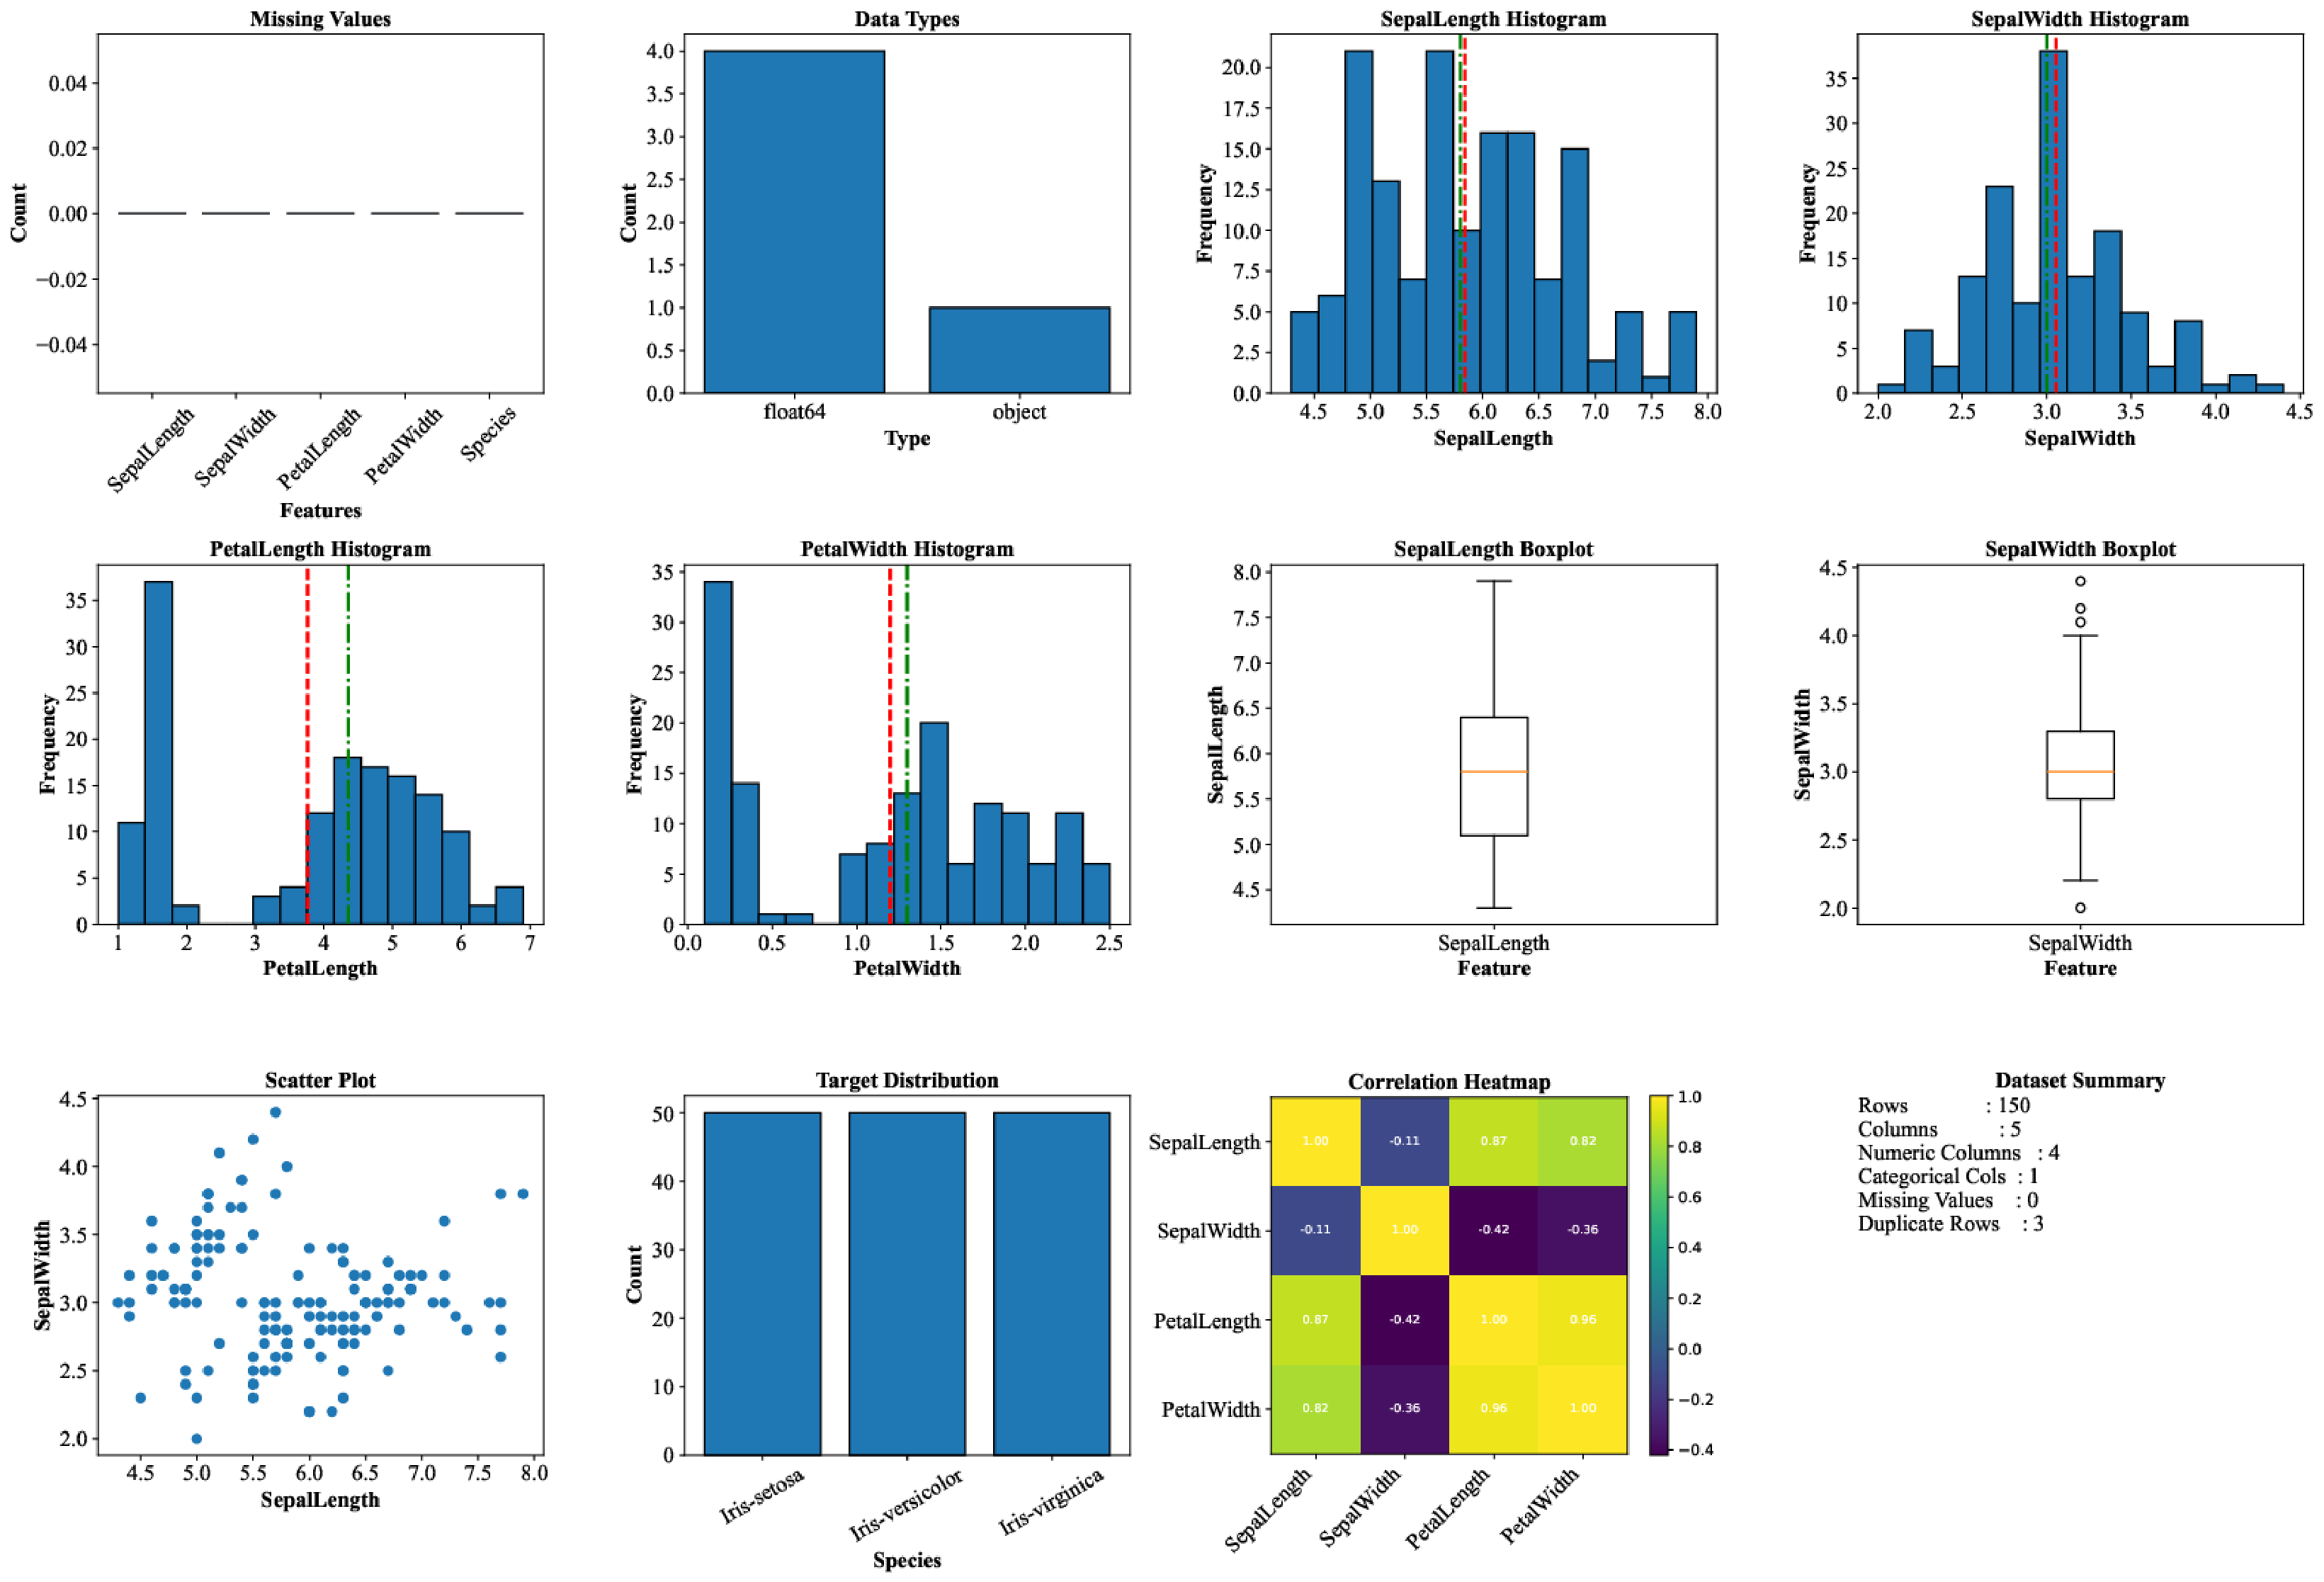
\includegraphics[width=\linewidth]{iris_eda.pdf}
\caption{Consolidated Exploratory Data Analysis of the Iris Dataset}
\end{figure}

\textbf{Inference:}

The Iris EDA summary confirms that the dataset is clean, with no missing values and only 3 duplicate rows out of 150 samples. Petal Length and Petal Width show the clearest visual separation between the three species, with \textit{Iris-setosa} forming a distinctly separable cluster from \textit{Iris-versicolor} and \textit{Iris-virginica}. Sepal measurements show more overlap between classes, particularly between the latter two species. This confirms that a well-chosen subset of features (particularly the petal measurements) carries strong discriminative power, which explains the high accuracy achieved by all four classifiers in this experiment.

\subsection{Diabetes Dataset EDA}

The exploratory data analysis of the Diabetes dataset was performed using four visualizations: an EDA summary figure, a correlation heatmap, feature distribution histograms, and boxplot analysis. These visualizations provide insights into feature relationships, data distributions, class characteristics, and potential outliers present in the dataset.

\begin{figure}[H]
\centering
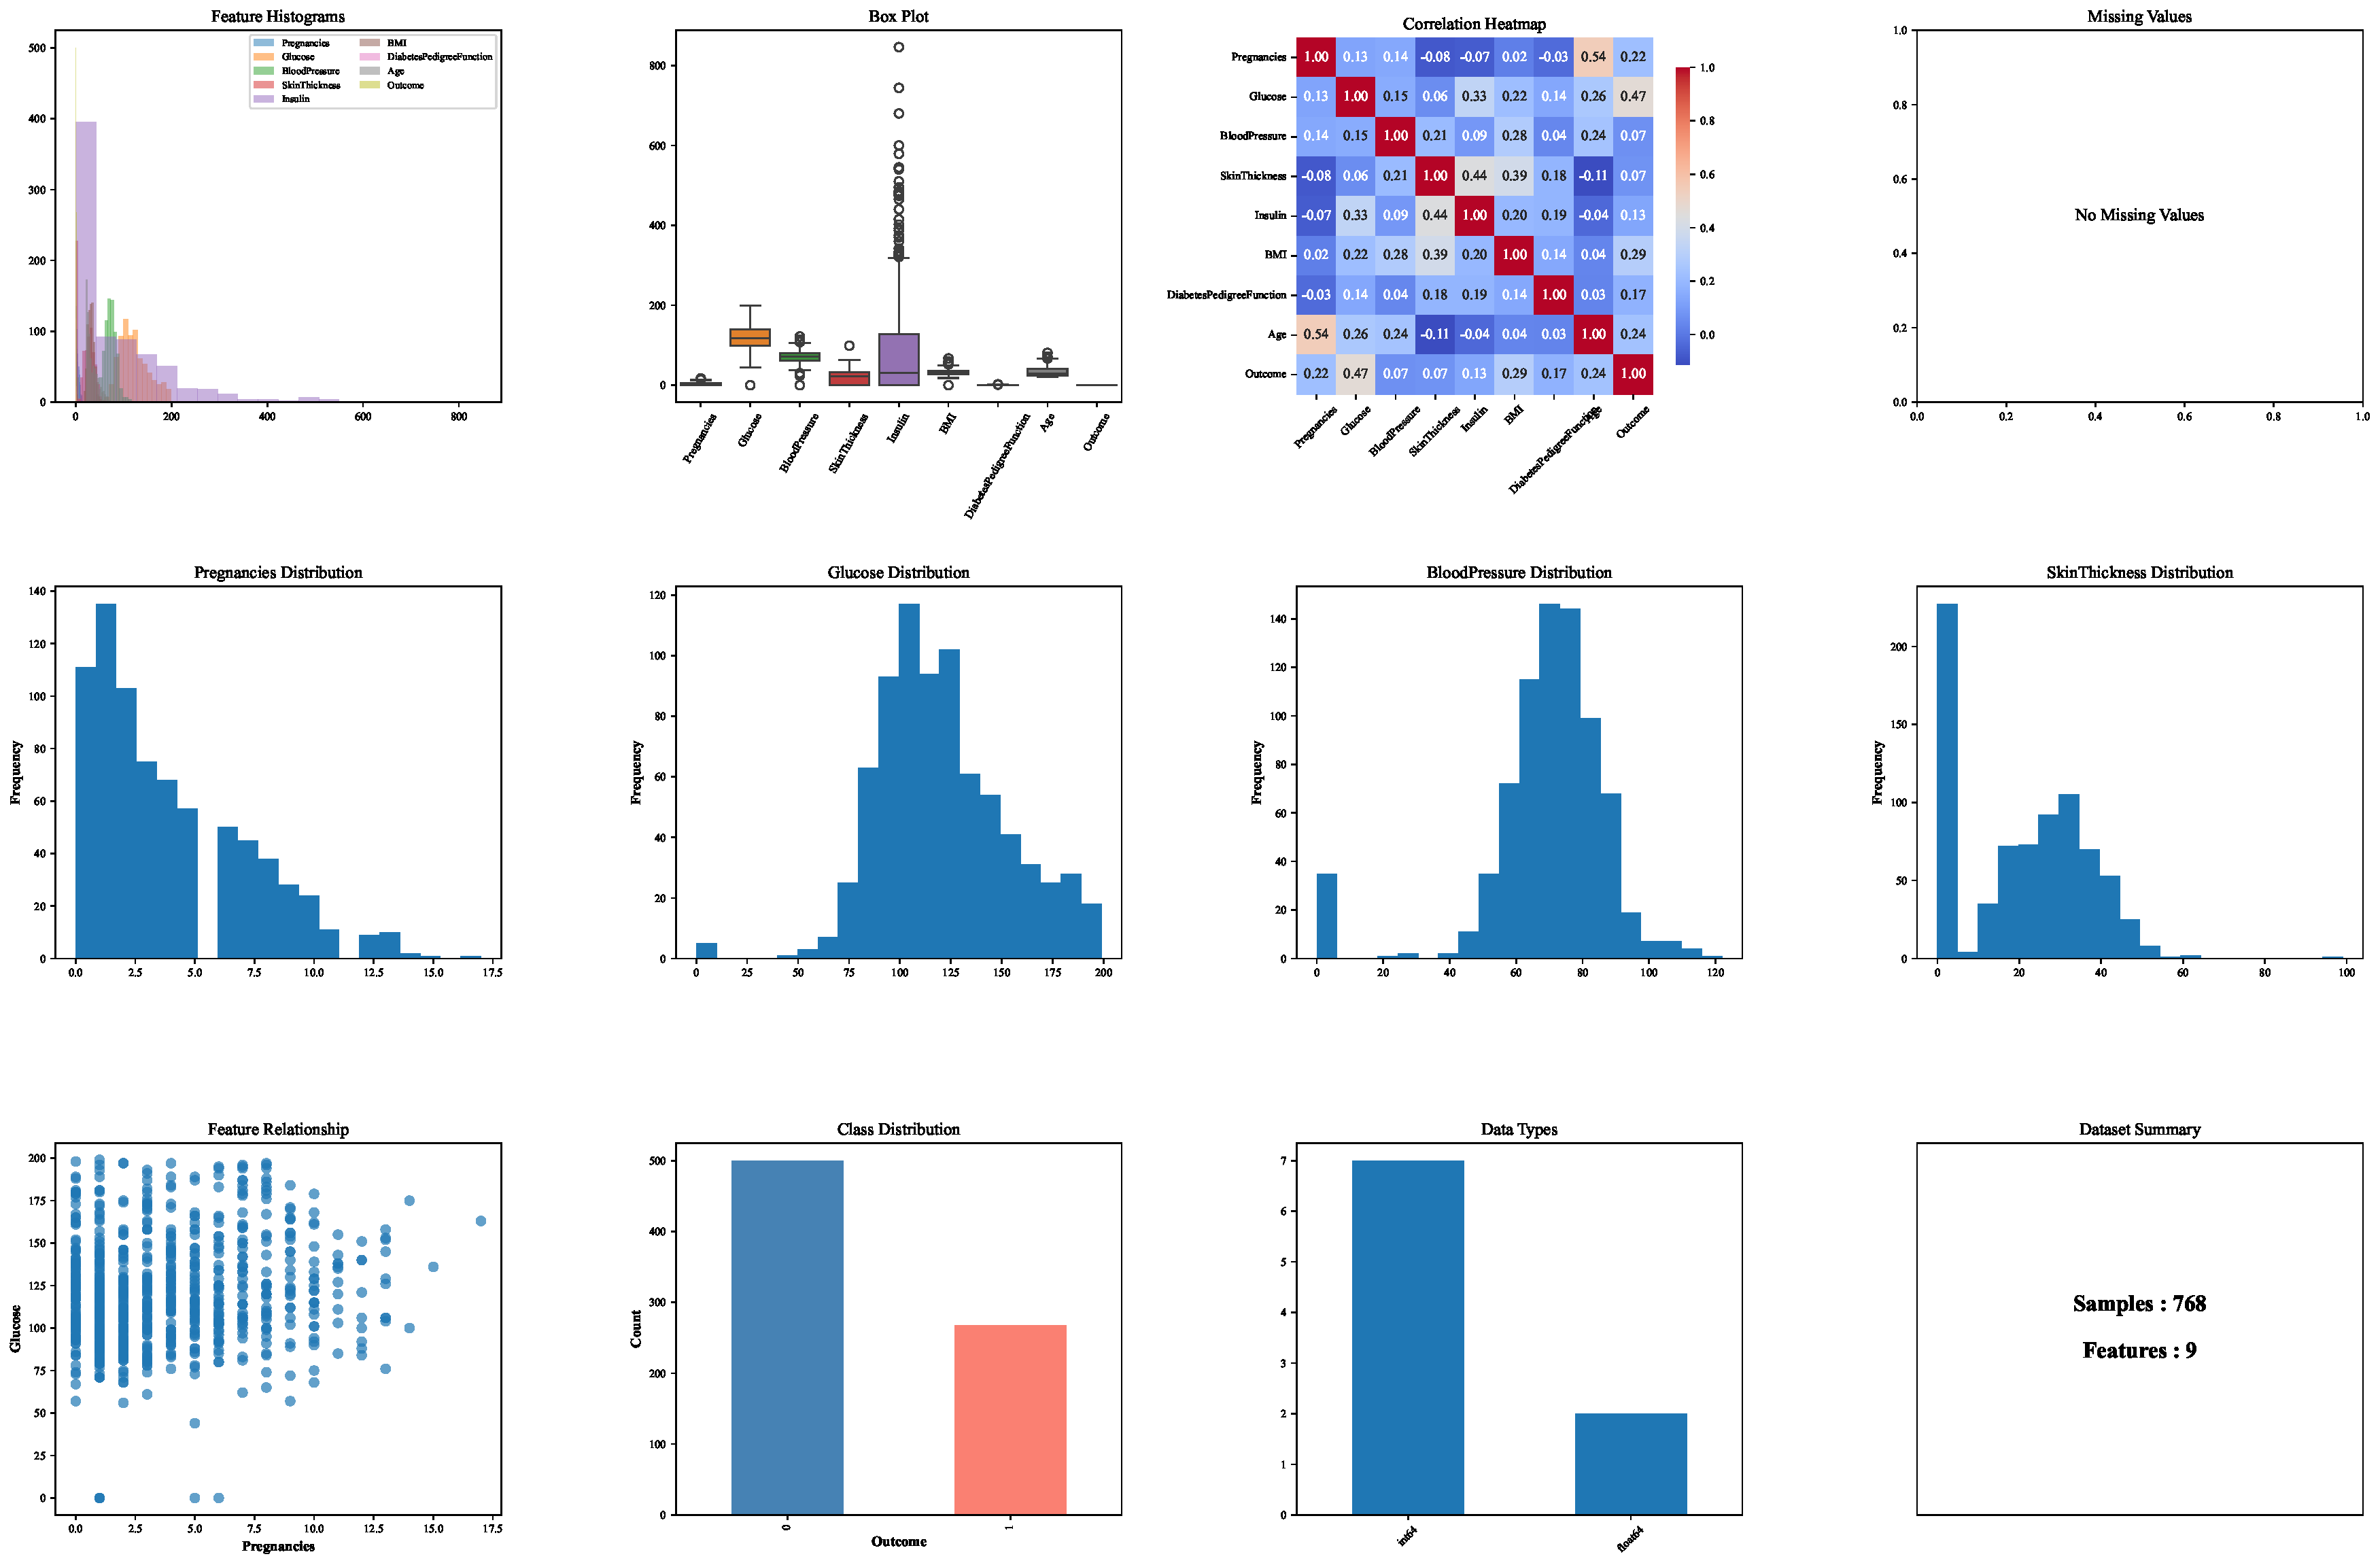
\includegraphics[width=\linewidth]{dataset_eda_1.pdf}
\caption{Comprehensive Exploratory Data Analysis of the Diabetes Dataset}
\end{figure}

\textbf{Inference:}

The EDA summary figure presents a consolidated overview of the Diabetes dataset containing 768 patient records and 9 attributes. The visualization includes dataset structure, statistical summary, class distribution, missing value analysis, feature relationships, and feature distributions. The analysis confirms that the dataset contains no missing values and is suitable for machine learning applications. Medical attributes such as Glucose, BMI, and Age appear to have a significant impact on diabetes prediction.

\begin{figure}[H]
\centering
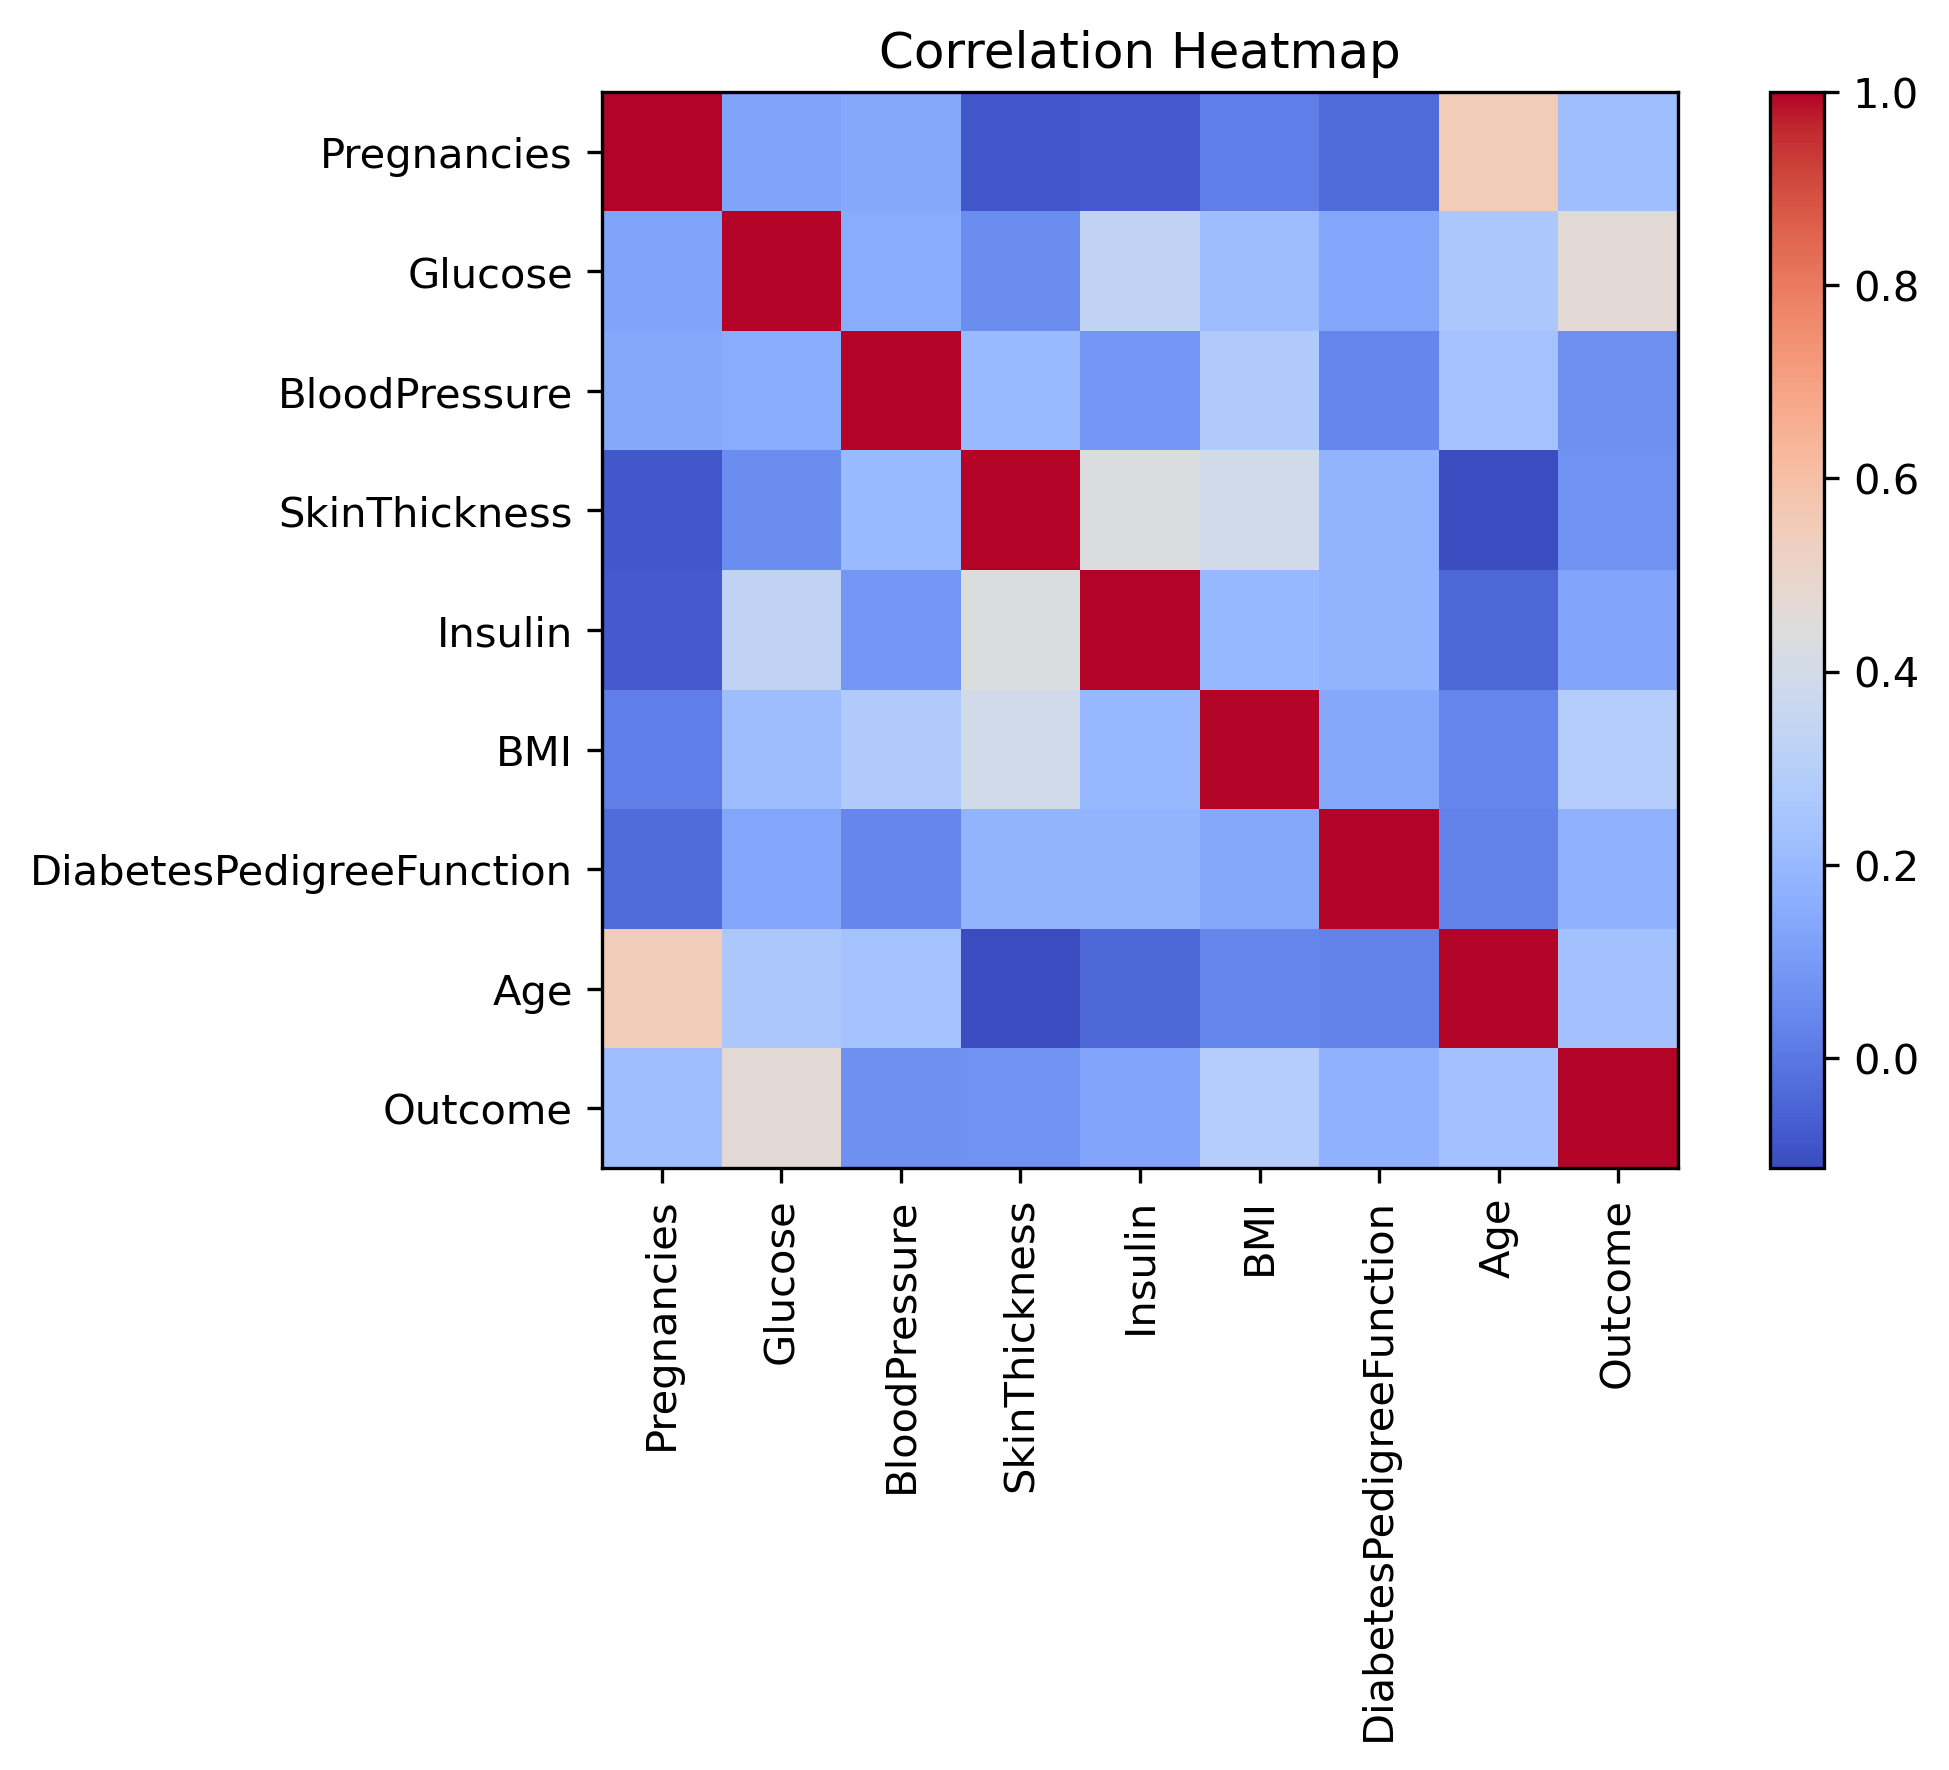
\includegraphics[width=0.8\linewidth]{heatmap1.png}
\caption{Correlation Heatmap of Diabetes Dataset Features}
\end{figure}

\textbf{Inference:}

The heatmap illustrates the correlation between different medical variables in the Diabetes dataset. Glucose exhibits the strongest positive relationship with the Outcome variable, indicating its importance in diabetes prediction. BMI and Age also show moderate positive correlations with the target class. The heatmap helps identify influential features that contribute to classification performance.

\begin{figure}[H]
\centering
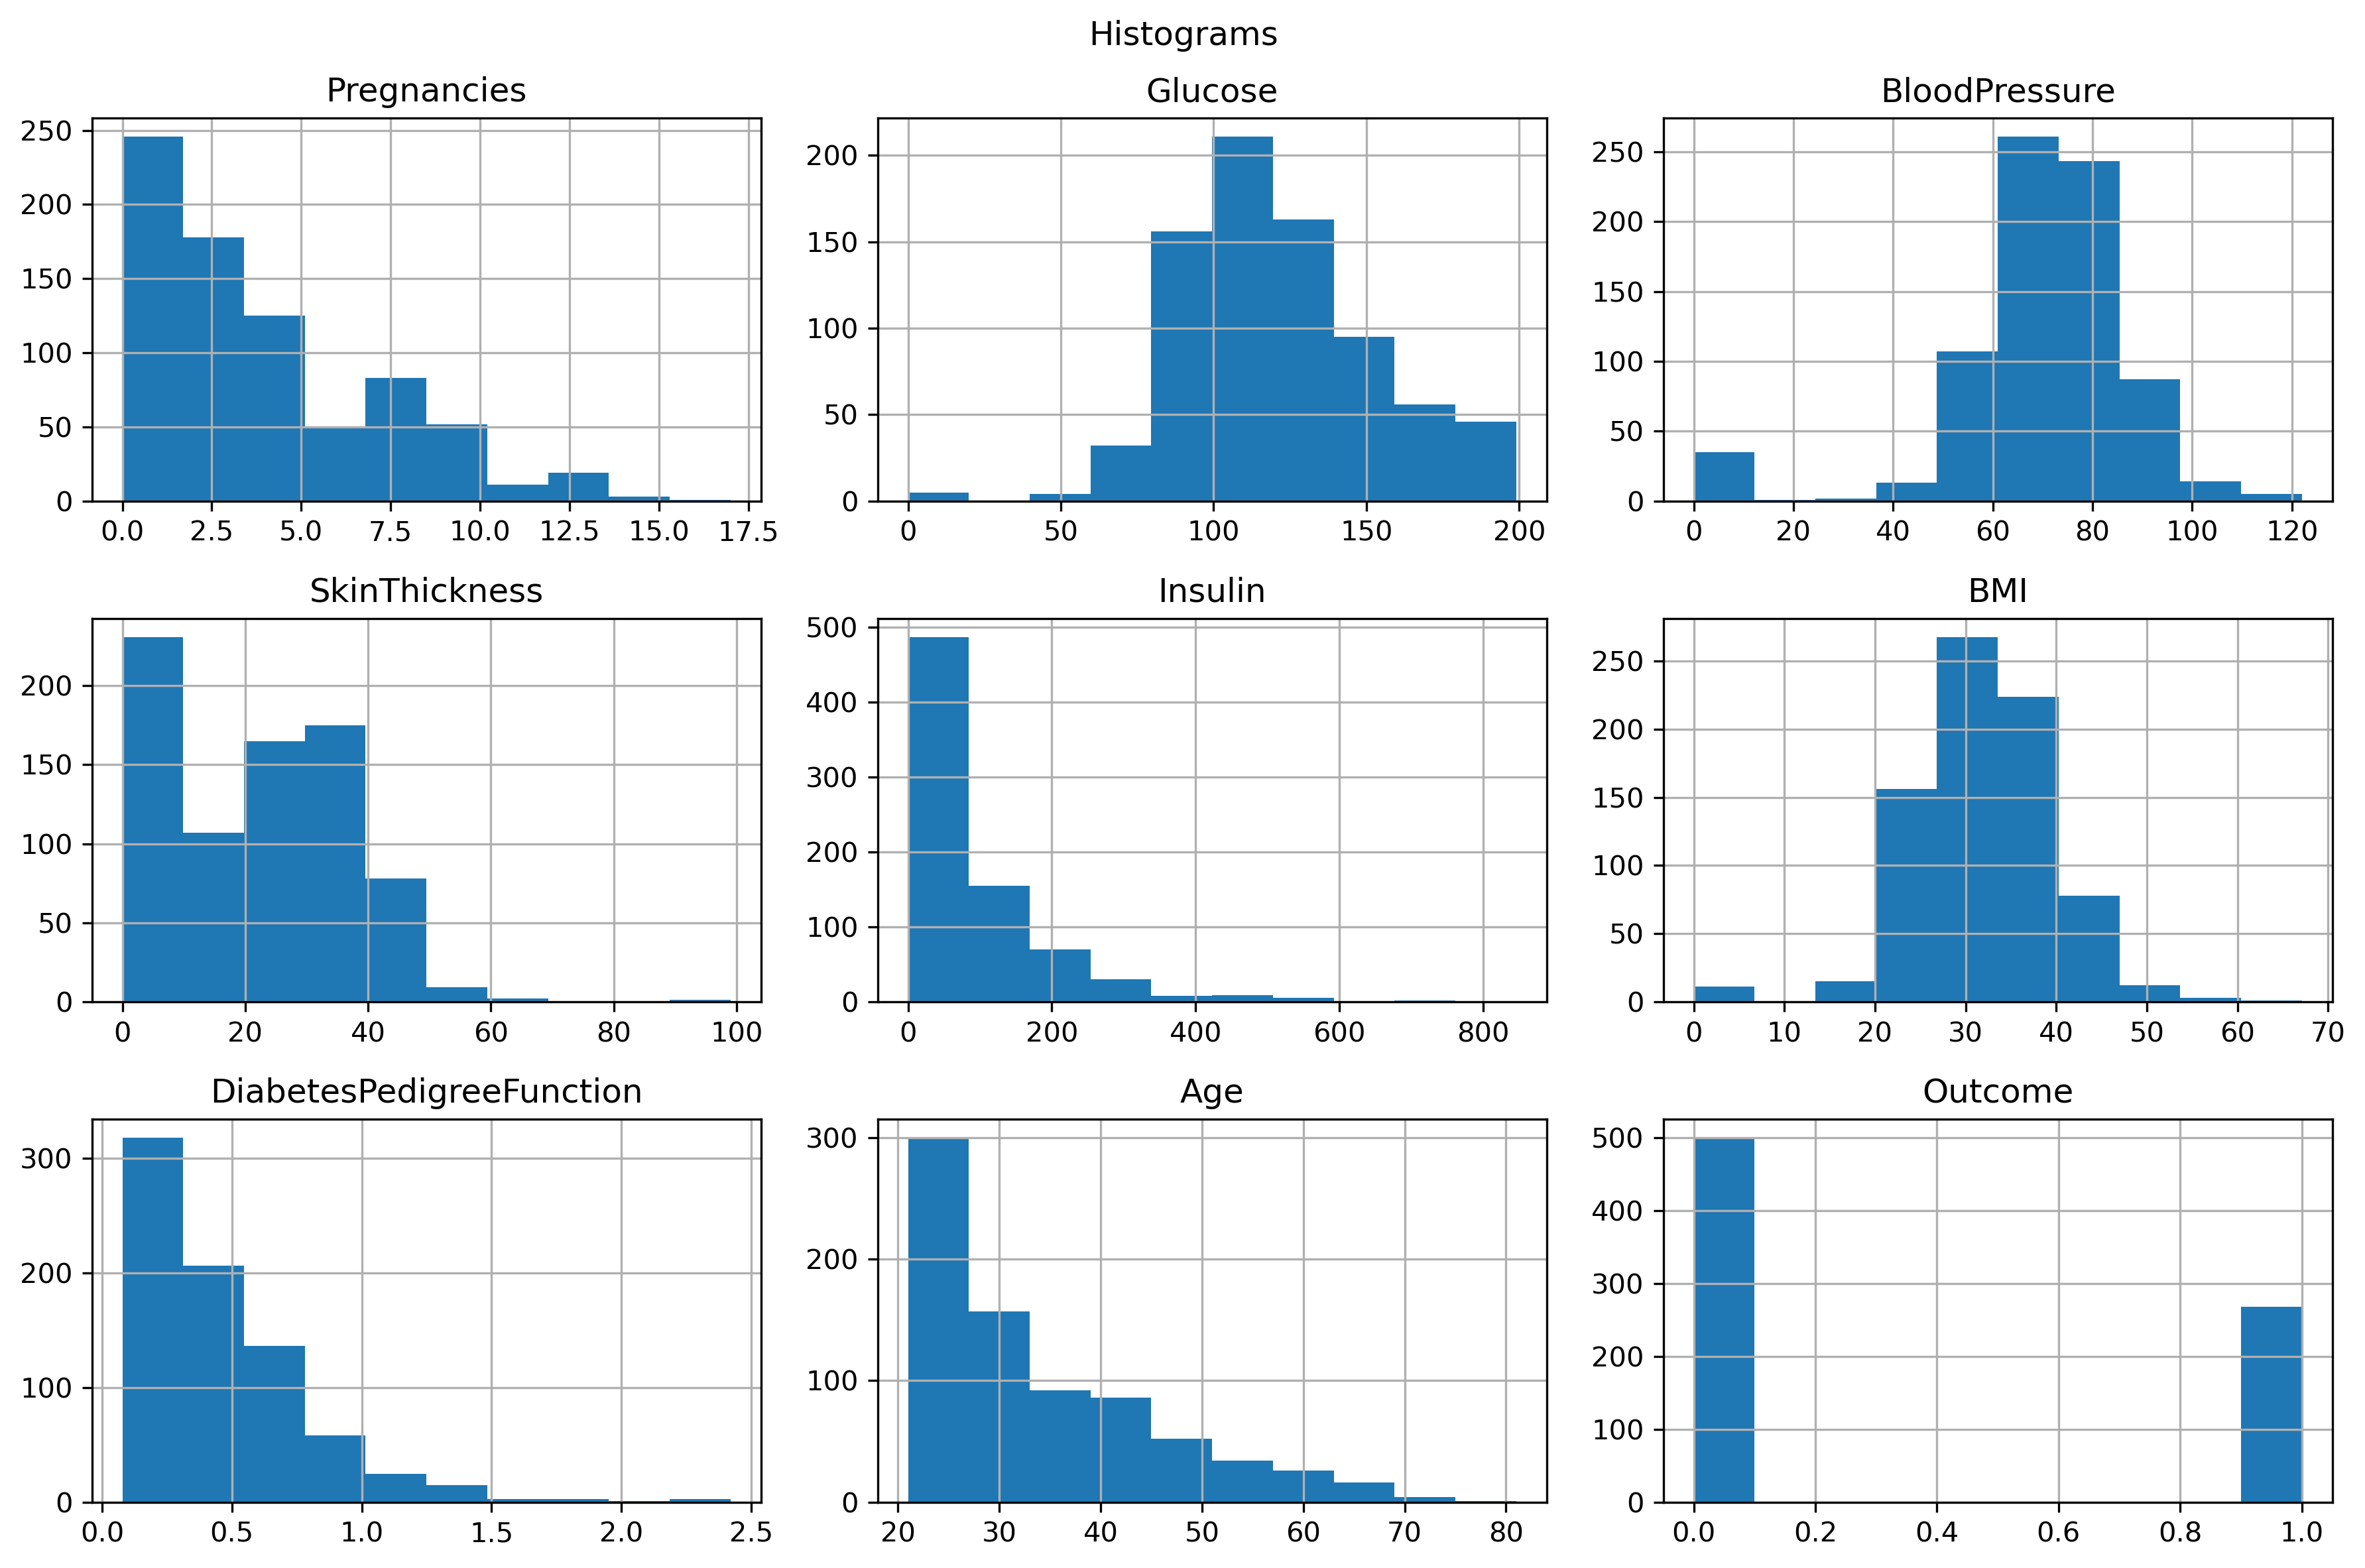
\includegraphics[width=0.8\linewidth]{histogram1.png}
\caption{Feature Distribution Histograms of the Diabetes Dataset}
\end{figure}

\textbf{Inference:}

The histogram visualization shows the distribution of numerical features such as Pregnancies, Glucose, Blood Pressure, Insulin, BMI, and Age. Several attributes exhibit skewed distributions and variability among patients. The distributions provide insight into the range and spread of medical measurements within the dataset. Understanding feature distributions is important for preprocessing and model development.

\begin{figure}[H]
\centering
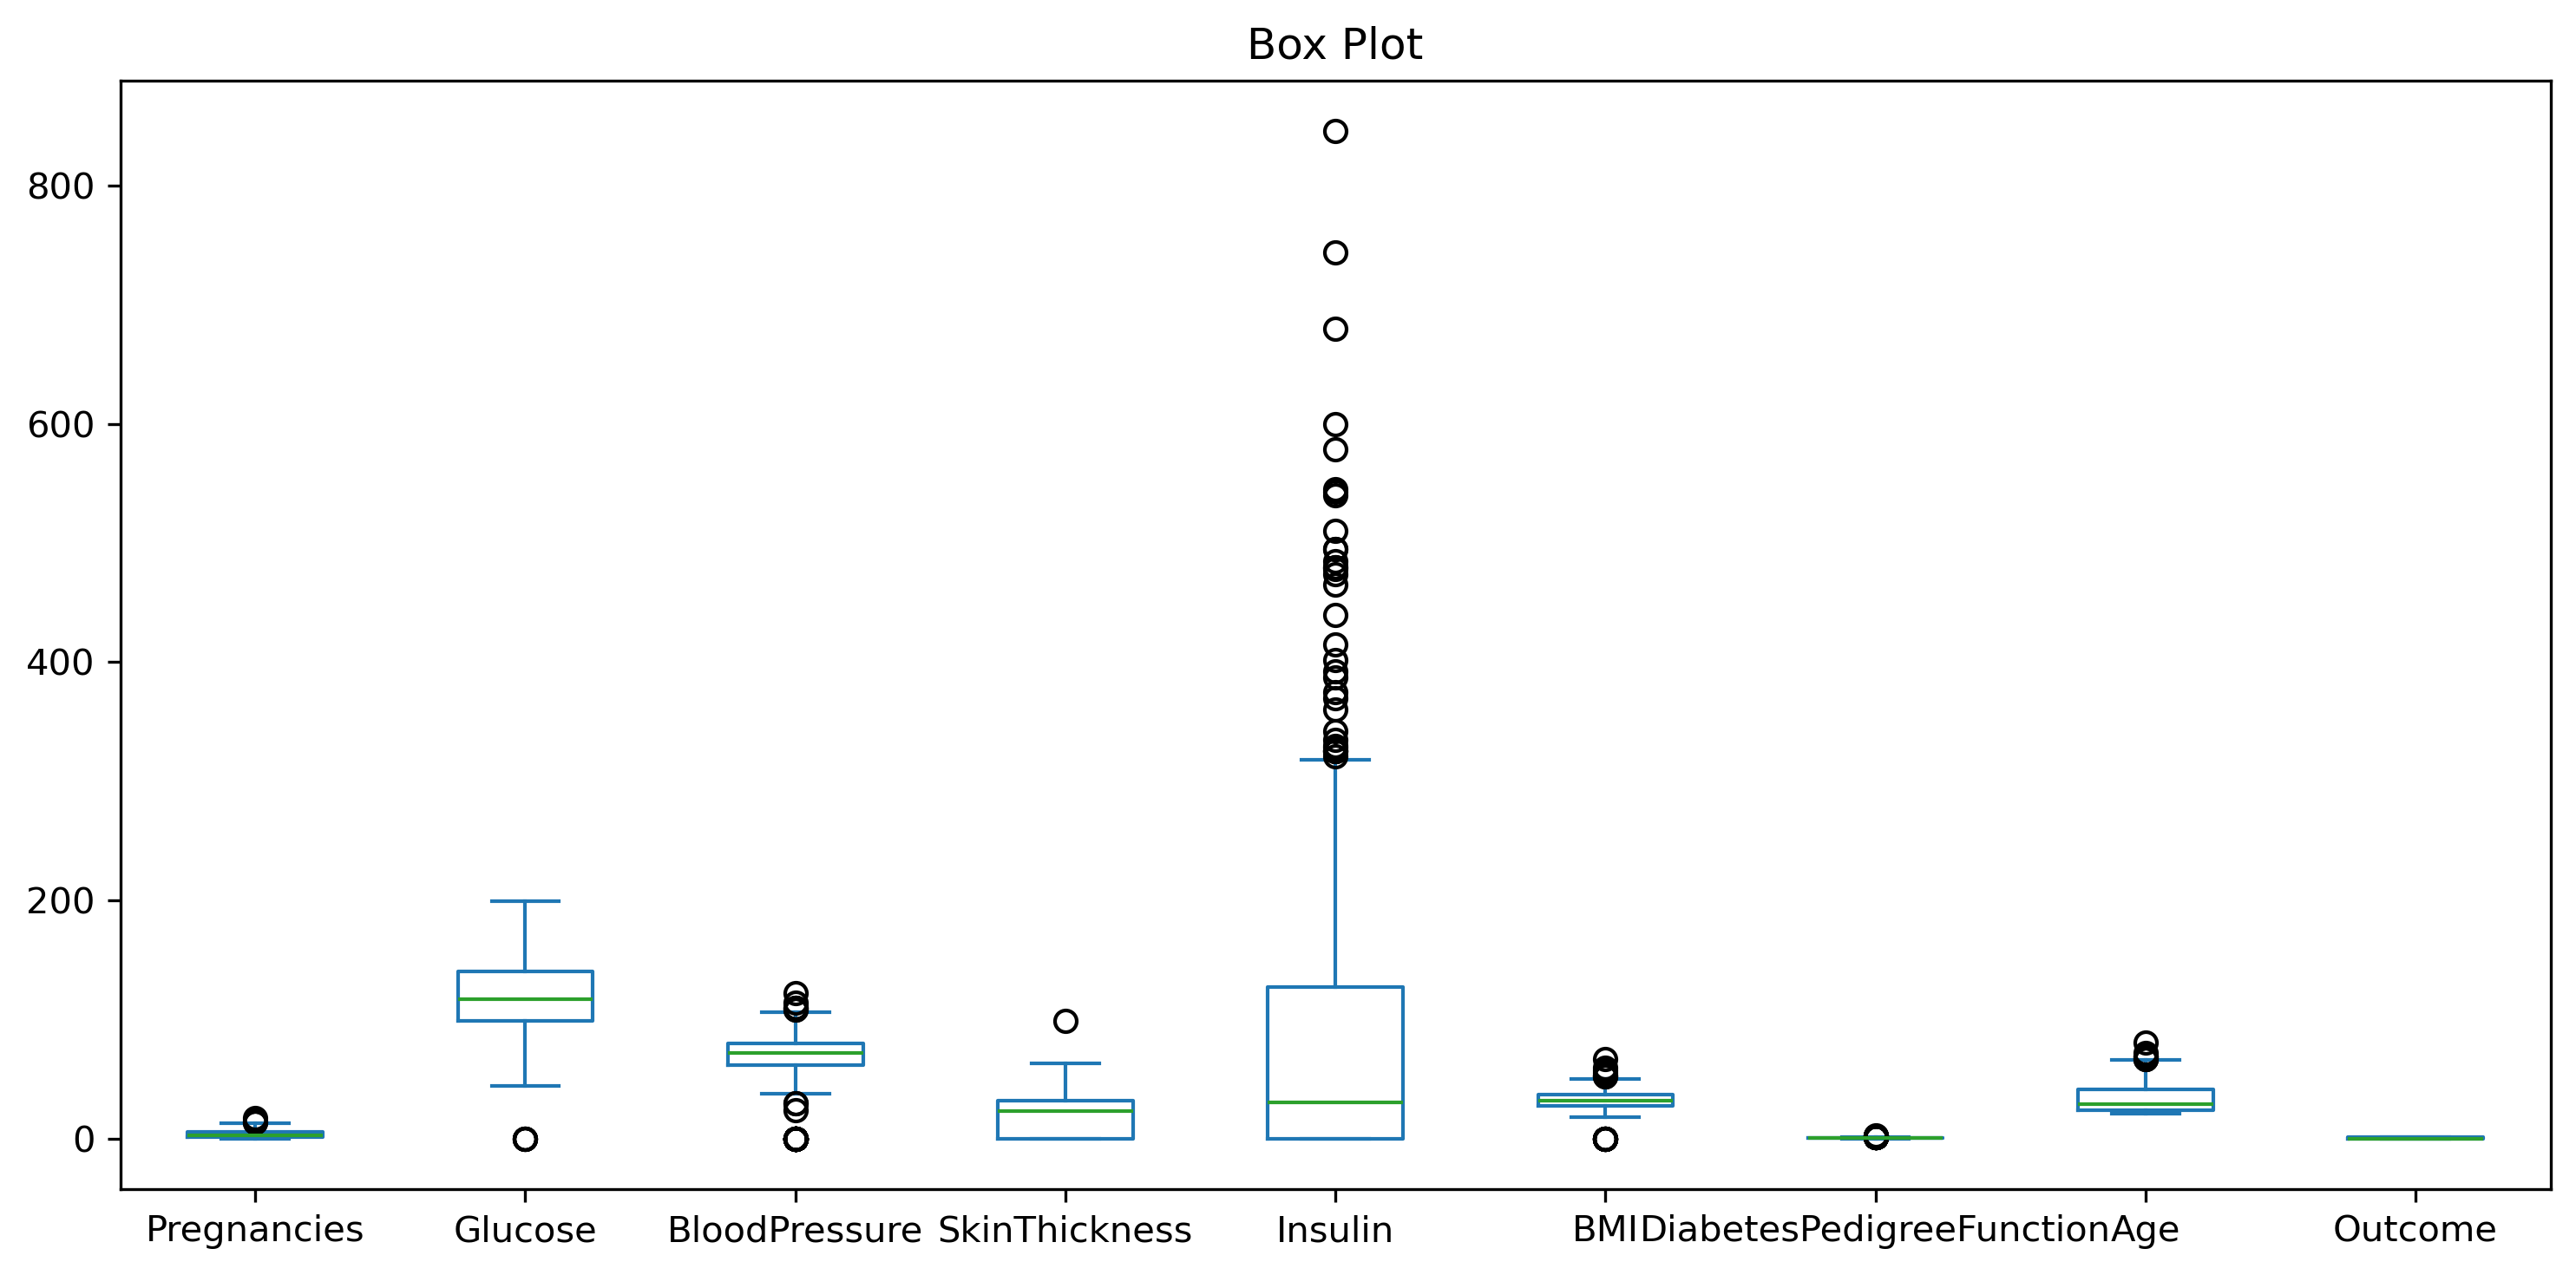
\includegraphics[width=0.8\linewidth]{boxplot1.png}
\caption{Boxplot Analysis of Diabetes Dataset Features}
\end{figure}

\textbf{Inference:}

The boxplots highlight the spread, median values, and potential outliers present in the dataset. Features such as Insulin and Glucose contain several extreme observations compared to other variables. The visualization helps identify variability in patient measurements and supports exploratory data analysis. Outlier detection is important for understanding model behavior and data quality.

\section{Data Preprocessing}

\subsection{Iris Dataset}

The Iris dataset's categorical \texttt{Species} column was label-encoded into numerical class values ($0$, $1$, $2$) to be compatible with Scikit-learn estimators. All four numerical features were standardized using \texttt{StandardScaler}:
\[
X_{scaled} = \frac{X - \mu}{\sigma}
\]
where $\mu$ is the feature mean and $\sigma$ is the feature standard deviation across the training set. Standardization is essential here because KNN and SVM are both distance/margin-based algorithms whose behavior is sensitive to the relative scale of Sepal and Petal measurements.

The dataset was then split into training and testing sets using an 80/20 stratified split (\texttt{random\_state=42}) to preserve equal class proportions across both sets, followed by ANOVA F-test based feature selection.

\subsubsection*{ANOVA F-test Feature Selection}

For each feature, the one-way ANOVA F-statistic measures how well that feature separates the $k$ target classes by comparing between-class variance to within-class variance:
\[
F = \frac{\text{Between-group variability}}{\text{Within-group variability}} = \frac{\sum_{j=1}^{k} n_j (\bar{x}_j - \bar{x})^2 / (k-1)}{\sum_{j=1}^{k}\sum_{i=1}^{n_j}(x_{ij}-\bar{x}_j)^2 / (N-k)}
\]
where $\bar{x}_j$ is the mean of feature $x$ within class $j$, $\bar{x}$ is the overall mean, $n_j$ is the number of samples in class $j$, and $N$ is the total sample count. A higher $F$-value indicates that a feature's means differ more strongly across classes relative to within-class spread, and is therefore more discriminative. In this experiment, \texttt{method="anova"} with \texttt{k="all"} was used, meaning all four features were ranked but none were dropped, allowing all classifiers to make use of the complete feature set while still benefiting from the relevance ranking internally.

\begin{table}[H]
\centering
\begin{tabular}{lc}
\toprule
Dataset & Samples \\
\midrule
Training Data & 120 \\
Testing Data & 30 \\
\bottomrule
\end{tabular}
\caption{Iris Train-Test Dataset Distribution}
\end{table}

\subsection{Diabetes Dataset}

The Diabetes dataset contains no categorical columns and no missing values, so preprocessing consisted of feature scaling (same standardization formula as above) followed by a train/validation/test split executed through the reusable \texttt{run\_pipeline()} function, using Random Forest as the classification algorithm and ANOVA as the feature-selection method.

\begin{table}[H]
\centering
\begin{tabular}{lc}
\toprule
Dataset & Samples \\
\midrule
Training Data & 491 \\
Validation Data & 123 \\
Testing Data & 154 \\
\bottomrule
\end{tabular}
\caption{Diabetes Train-Validation-Test Dataset Distribution}
\end{table}

\section{Implementation Details}

The workflow was modularized into reusable functions organized into dedicated source modules (\texttt{data\_loader.py}, \texttt{utils.py}, \texttt{eda.py}, \texttt{preprocessing.py}, \texttt{feature\_selection.py}, \texttt{classification.py}, \texttt{metrics.py}, \texttt{main.py}):

\begin{itemize}
\item \texttt{load\_dataset()} -- loads a CSV dataset and prints a shape/summary confirmation.
\item \texttt{dataset\_info()} -- prints shape, column names, data types, missing values, duplicate rows, and summary statistics.
\item \texttt{perform\_eda()} -- generates the consolidated EDA summary figure for a given dataset and target column.
\item \texttt{preprocess\_data()} -- performs encoding, scaling, and stratified train-test splitting.
\item \texttt{select\_features()} -- performs ANOVA F-test based feature selection/ranking.
\item \texttt{train\_classification()} -- trains a specified classification algorithm (Random Forest, Decision Tree, KNN, SVM).
\item \texttt{classification\_metrics()} -- computes Accuracy, Precision, Recall, F1-Score, Confusion Matrix, Classification Report, and ROC-AUC.
\item \texttt{run\_pipeline()} -- an end-to-end wrapper that chains loading, preprocessing, and model training/evaluation for quick experimentation on any dataset by changing only the dataset path and target column.
\end{itemize}

This modular design allowed the exact same code to be reused across the Iris and Diabetes datasets by changing only the dataset path and target column name, validating the goal of building a general-purpose ML pipeline.

\section{Machine Learning Algorithms}

Four classification algorithms were used across the two datasets in this experiment. Their working principles and mathematical formulations are detailed below.

\subsection{Random Forest}

Random Forest is an ensemble learning method that constructs $T$ decision trees, each trained on an independent bootstrap sample of the training data (bagging), with each split additionally restricted to a random subset of $m$ features (typically $m = \sqrt{p}$ for classification, where $p$ is the total feature count). For a new sample $x$, each tree $t$ produces a class prediction $h_t(x)$, and the forest predicts the majority class:
\[
\hat{y} = \text{mode}\{h_1(x), h_2(x), \dots, h_T(x)\}
\]
Each individual tree is grown by recursively splitting nodes to minimize \textbf{Gini impurity}:
\[
G = 1 - \sum_{i=1}^{k} p_i^2
\]
where $p_i$ is the proportion of samples belonging to class $i$ at that node, and $k$ is the number of classes. By averaging over many de-correlated trees, Random Forest reduces the variance associated with any single decision tree without significantly increasing bias.

\textbf{Advantages:} Robust to overfitting; handles non-linear relationships well; provides feature importance estimates; requires little preprocessing.

\textbf{Limitations:} Less interpretable than a single decision tree; can be computationally heavier for large forests; prediction time scales with the number of trees.

\subsection{Decision Tree}

A Decision Tree recursively partitions the feature space into regions that maximize class purity at each split. Two common splitting criteria are Gini impurity (defined above) and \textbf{entropy}:
\[
H = -\sum_{i=1}^{k} p_i \log_2(p_i)
\]
At each node, the algorithm selects the feature and threshold that maximize the \textbf{information gain}:
\[
IG = H(\text{parent}) - \sum_{c \in \{\text{left, right}\}} \frac{n_c}{n} H(c)
\]
where $n_c$ is the number of samples in child node $c$ and $n$ is the number of samples in the parent node. This process repeats recursively until a stopping criterion (e.g. maximum depth, minimum samples per leaf) is reached, producing a hierarchical set of if-else decision rules.

\textbf{Advantages:} Highly interpretable; requires no feature scaling; handles both numerical and categorical data naturally.

\textbf{Limitations:} Prone to overfitting on training data if not pruned or depth-limited; unstable to small changes in the data (high variance).

\subsection{K-Nearest Neighbors (KNN)}

KNN is a non-parametric, instance-based algorithm that classifies a query sample $x$ based on the majority class among its $k$ nearest neighbors in feature space, most commonly using \textbf{Euclidean distance}:
\[
d(x, x_i) = \sqrt{\sum_{j=1}^{p}(x_j - x_{ij})^2}
\]
where $p$ is the number of features. Given the $k$ nearest training points $\{x_{(1)}, \dots, x_{(k)}\}$ to $x$ (sorted by increasing distance), the predicted class is:
\[
\hat{y} = \text{mode}\{y_{(1)}, y_{(2)}, \dots, y_{(k)}\}
\]
Since KNN relies entirely on distance computation, feature scaling (as applied in preprocessing) is critical -- unscaled features with larger numeric ranges would otherwise dominate the distance calculation.

\textbf{Advantages:} Simple and intuitive; naturally handles multi-class problems; no explicit training phase (lazy learning).

\textbf{Limitations:} Computationally expensive at prediction time for large datasets ($O(n)$ per query); sensitive to feature scaling and irrelevant features; performance depends heavily on the choice of $k$.

\subsection{Support Vector Machine (SVM)}

SVM constructs the hyperplane that maximizes the margin between classes:
\[
f(x) = w^Tx + b
\]
For the soft-margin formulation, the optimization problem is:
\[
\min_{w,b,\xi} \; \frac{1}{2}\|w\|^2 + C\sum_{i=1}^{n}\xi_i \quad \text{subject to} \quad y_i(w^Tx_i+b) \geq 1-\xi_i,\ \xi_i \geq 0
\]
where $C$ controls the trade-off between maximizing the margin $\frac{2}{\|w\|}$ and minimizing misclassification via the slack variables $\xi_i$. For non-linearly separable classes (as with the three-way Iris boundary), SVM implicitly maps inputs into a higher-dimensional space via a kernel function $K(x_i, x_j)$, most commonly the RBF kernel $K(x_i,x_j) = \exp(-\gamma\|x_i-x_j\|^2)$, without explicitly computing the transformation (the ``kernel trick''). A fuller kernel-by-kernel treatment of SVM is provided in Experiment 4 of this laboratory series.

\textbf{Advantages:} Effective in high-dimensional spaces; robust to overfitting with proper regularization; kernel trick enables non-linear decision boundaries.

\textbf{Limitations:} Less interpretable; sensitive to hyperparameter and kernel choice; does not natively output class probabilities.

\section{Experimental Setup}

\begin{table}[H]
\centering
\begin{tabular}{ll}
\toprule
Parameter & Details \\
\midrule
Programming Language & Python 3.14 \\
Machine Learning Library & Scikit-Learn 1.4.2 \\
Data Processing Library & Pandas 2.2.2, NumPy 1.26.4 \\
Scientific Computing Library & SciPy 1.13.1 \\
Visualization Library & Matplotlib \\
Development Environment & Jupyter Notebook \\
Operating System & Windows / Linux (Anaconda Environment) \\
Iris Dataset Size & 150 samples \\
Diabetes Dataset Size & 768 samples \\
\bottomrule
\end{tabular}
\caption{Experimental Environment}
\end{table}

\section{Evaluation Metrics}

All classification results in this report are evaluated using the following metrics, defined in terms of True Positives (TP), True Negatives (TN), False Positives (FP), and False Negatives (FN):

\[
\text{Accuracy} = \frac{TP+TN}{TP+TN+FP+FN}
\]
\[
\text{Precision} = \frac{TP}{TP+FP}
\]
\[
\text{Recall} = \frac{TP}{TP+FN}
\]
\[
\text{F1-Score} = 2 \cdot \frac{\text{Precision} \cdot \text{Recall}}{\text{Precision}+\text{Recall}}
\]

For multi-class problems (as with Iris), each metric except accuracy is computed on a one-vs-rest basis per class, then combined via a weighted average (weighted by class support) as reported in the classification report.

\textbf{ROC-AUC:} The Receiver Operating Characteristic curve plots the True Positive Rate against the False Positive Rate at varying classification thresholds:
\[
TPR = \frac{TP}{TP+FN}, \qquad FPR = \frac{FP}{FP+TN}
\]
The Area Under the Curve (AUC) summarizes this curve into a single value between 0 and 1, representing the probability that the model ranks a randomly chosen positive sample above a randomly chosen negative sample. For the multi-class Iris problem, ROC-AUC is computed using the one-vs-rest (OvR) strategy and averaged across classes.

\section{Hyperparameter Selection}

The four Iris classifiers were run using standard Scikit-learn default hyperparameters (no exhaustive grid search was performed in this introductory experiment), as the goal was to validate library familiarity and pipeline reusability rather than optimal tuning. The Diabetes pipeline used Random Forest (\texttt{model\_name="rf"}) with ANOVA feature selection (\texttt{feature\_method="anova"}) via the \texttt{run\_pipeline()} default configuration.

\begin{table}[H]
\centering
\begin{tabular}{ll}
\toprule
Parameter & Value \\
\midrule
Iris -- Feature Selection Method & ANOVA F-test, $k=$ all \\
Iris -- Train/Test Split & 80/20, stratified, random\_state=42 \\
Diabetes -- Model & Random Forest (\texttt{rf}) \\
Diabetes -- Feature Selection Method & ANOVA \\
\bottomrule
\end{tabular}
\caption{Pipeline Configuration Parameters}
\end{table}

\section{Results -- Iris Dataset}

Four classification algorithms were trained and evaluated on the Iris test set (30 samples) after ANOVA-based feature selection.

\begin{table}[H]
\centering
\begin{tabular}{lcccc}
\toprule
Model & Accuracy & Precision & Recall & F1-Score \\
\midrule
Random Forest & 0.9667 & 0.9697 & 0.9667 & 0.9666 \\
Decision Tree & 0.9333 & 0.9333 & 0.9333 & 0.9333 \\
KNN & 0.9333 & 0.9444 & 0.9333 & 0.9327 \\
SVM & 0.9667 & 0.9697 & 0.9667 & 0.9666 \\
\bottomrule
\end{tabular}
\caption{Iris Dataset -- Classification Model Comparison}
\end{table}

\begin{table}[H]
\centering
\begin{tabular}{lc}
\toprule
Model & ROC-AUC (OvR) \\
\midrule
Random Forest & 0.9900 \\
Decision Tree & 0.9500 \\
KNN & 0.9933 \\
SVM & 0.9967 \\
\bottomrule
\end{tabular}
\caption{Iris Dataset -- ROC-AUC Comparison (One-vs-Rest)}
\end{table}

\subsection*{Random Forest}

\begin{table}[H]
\centering
\begin{tabular}{lccc}
\toprule
Class & Precision & Recall & F1-Score \\
\midrule
0 (setosa) & 1.00 & 1.00 & 1.00 \\
1 (versicolor) & 1.00 & 0.90 & 0.95 \\
2 (virginica) & 0.91 & 1.00 & 0.95 \\
\bottomrule
\end{tabular}
\caption{Random Forest -- Classification Report (Iris)}
\end{table}

Confusion Matrix: $\begin{bmatrix} 10 & 0 & 0 \\ 0 & 9 & 1 \\ 0 & 0 & 10 \end{bmatrix}$

\begin{figure}[H]
\centering
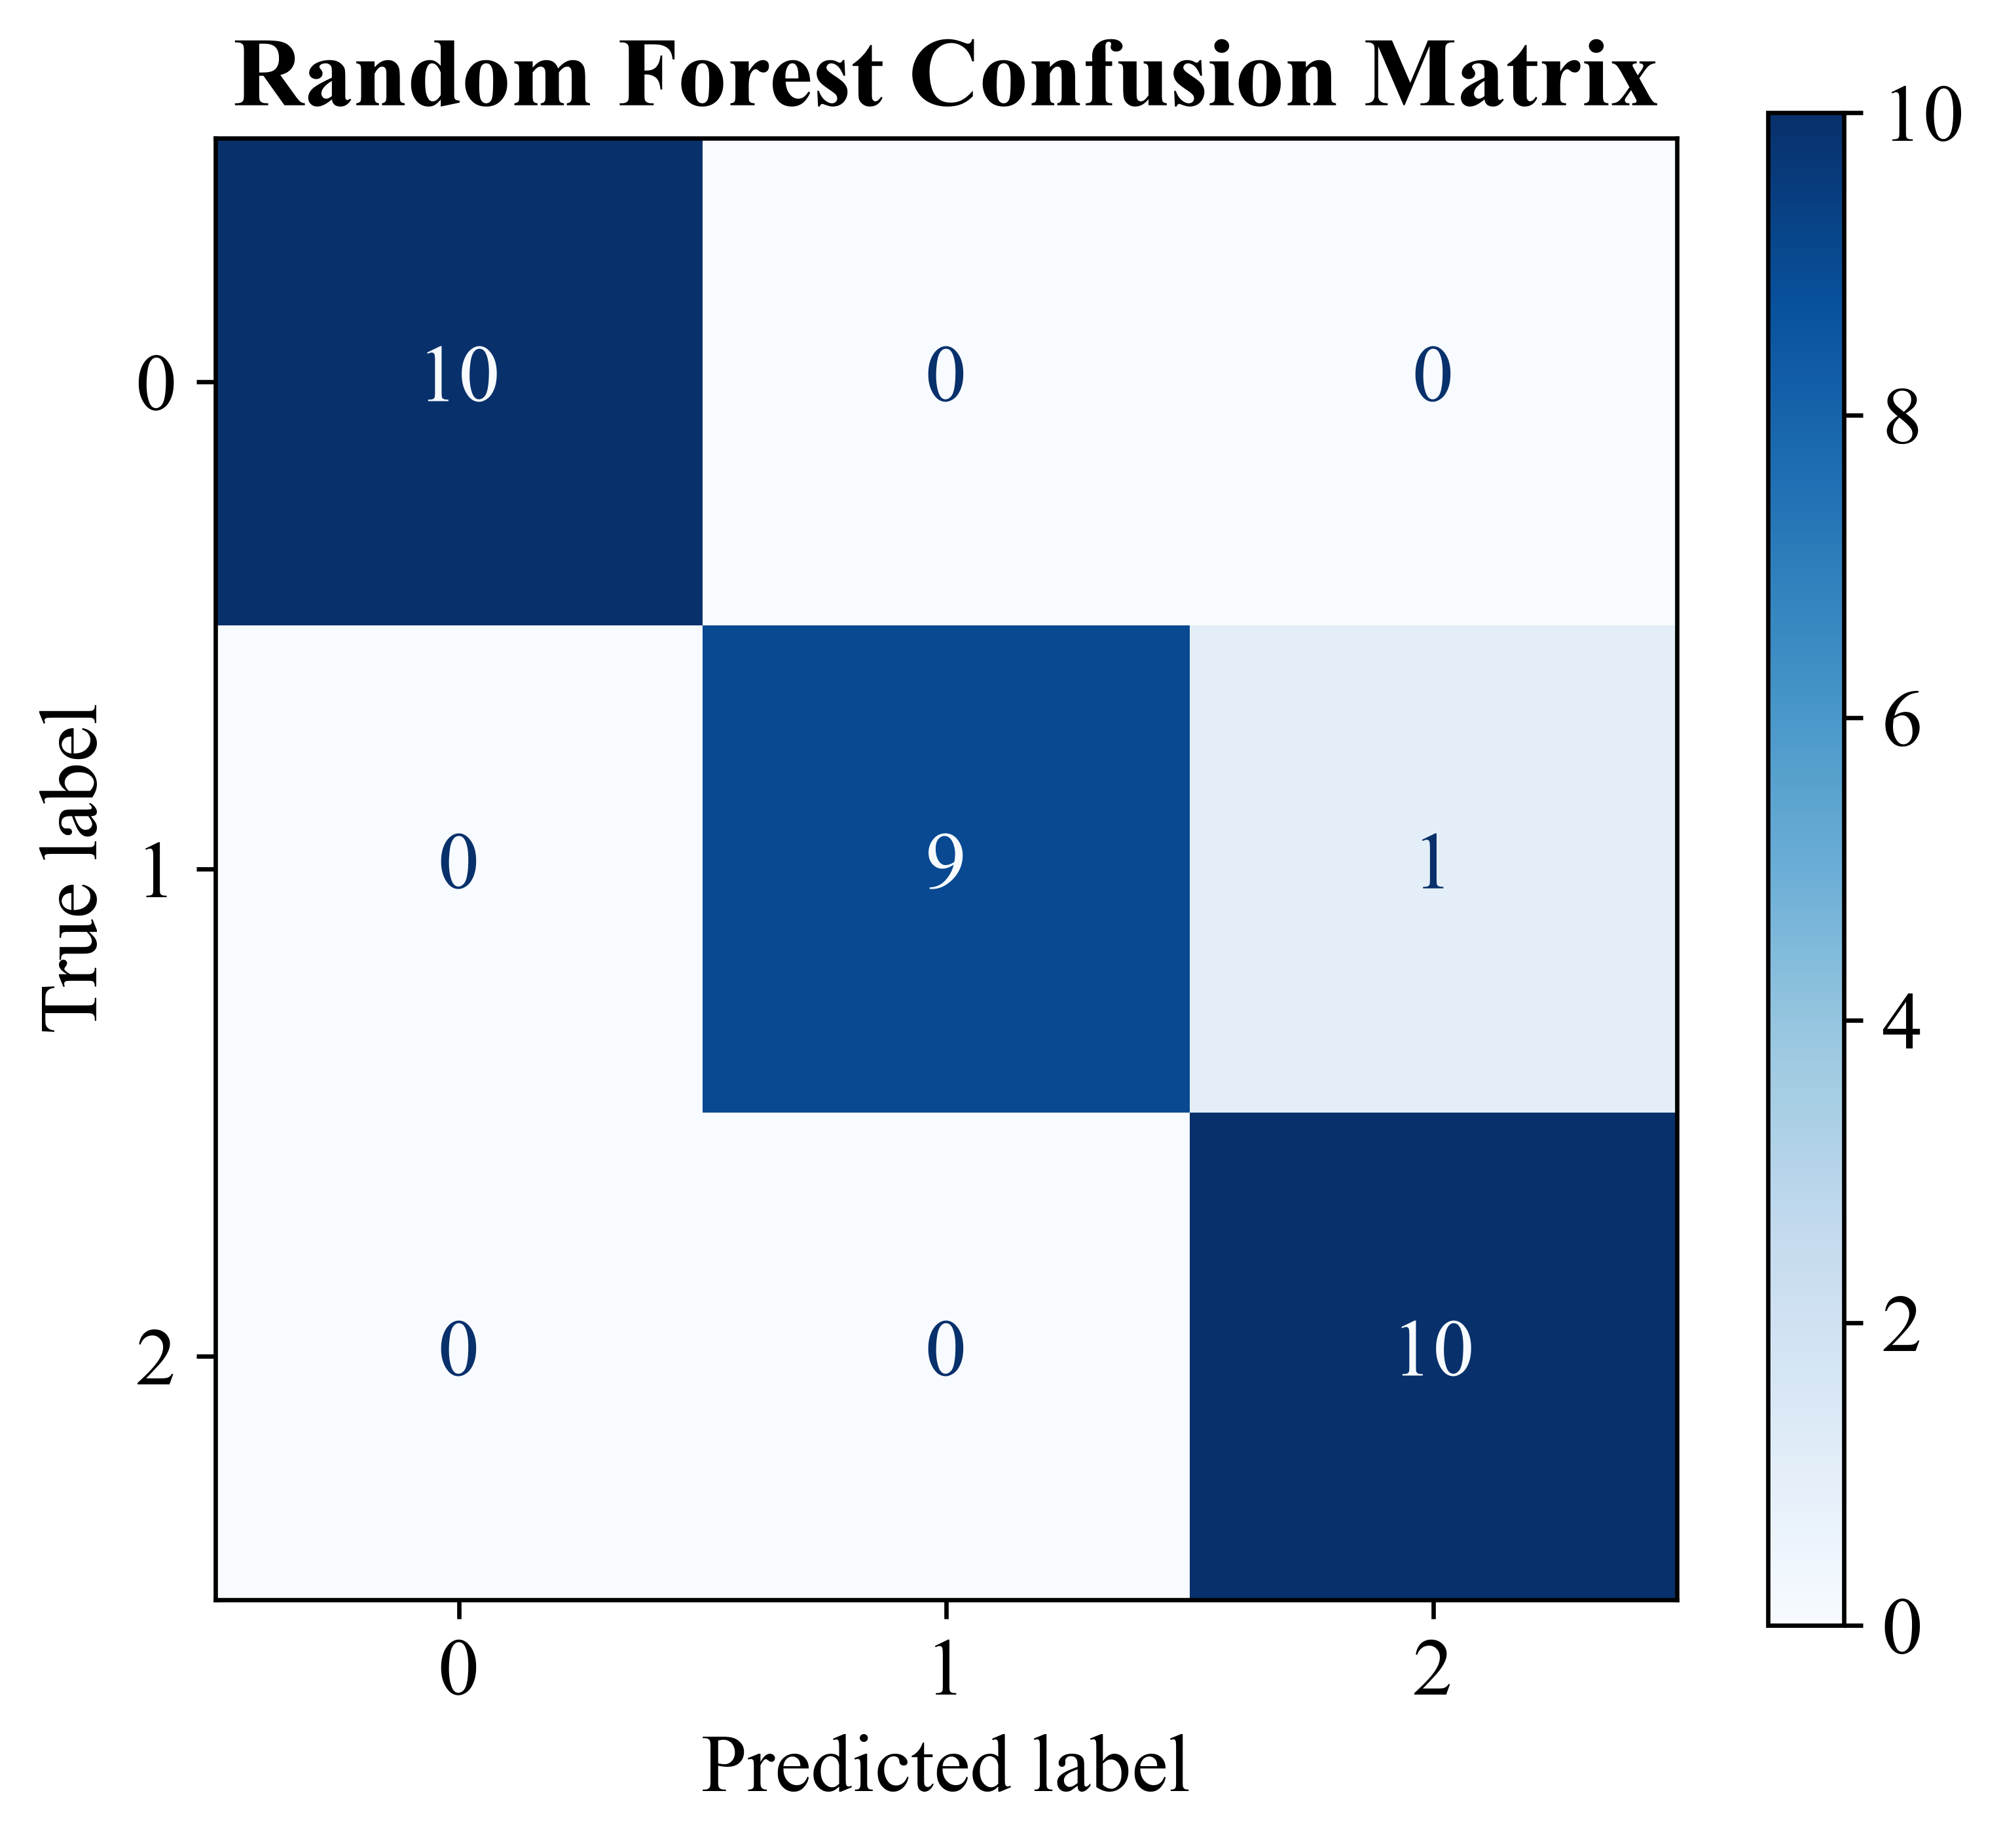
\includegraphics[width=0.55\linewidth]{random_forest_confusion_matrix.png}
\caption{Confusion Matrix -- Random Forest (Iris)}
\end{figure}

\textbf{Inference:} Random Forest achieves the joint-best accuracy (96.67\%) on the Iris test set, misclassifying only a single \textit{versicolor} sample as \textit{virginica} (visible as the off-diagonal entry in row 2). This confirms that averaging across bootstrapped, feature-randomized trees generalizes well even on this small, low-dimensional dataset, and that Gini-impurity-based splits successfully isolate the near-linear petal-based class boundaries.

\subsection*{Decision Tree}

\begin{table}[H]
\centering
\begin{tabular}{lccc}
\toprule
Class & Precision & Recall & F1-Score \\
\midrule
0 (setosa) & 1.00 & 1.00 & 1.00 \\
1 (versicolor) & 0.90 & 0.90 & 0.90 \\
2 (virginica) & 0.90 & 0.90 & 0.90 \\
\bottomrule
\end{tabular}
\caption{Decision Tree -- Classification Report (Iris)}
\end{table}

Confusion Matrix: $\begin{bmatrix} 10 & 0 & 0 \\ 0 & 9 & 1 \\ 0 & 1 & 9 \end{bmatrix}$

\begin{figure}[H]
\centering
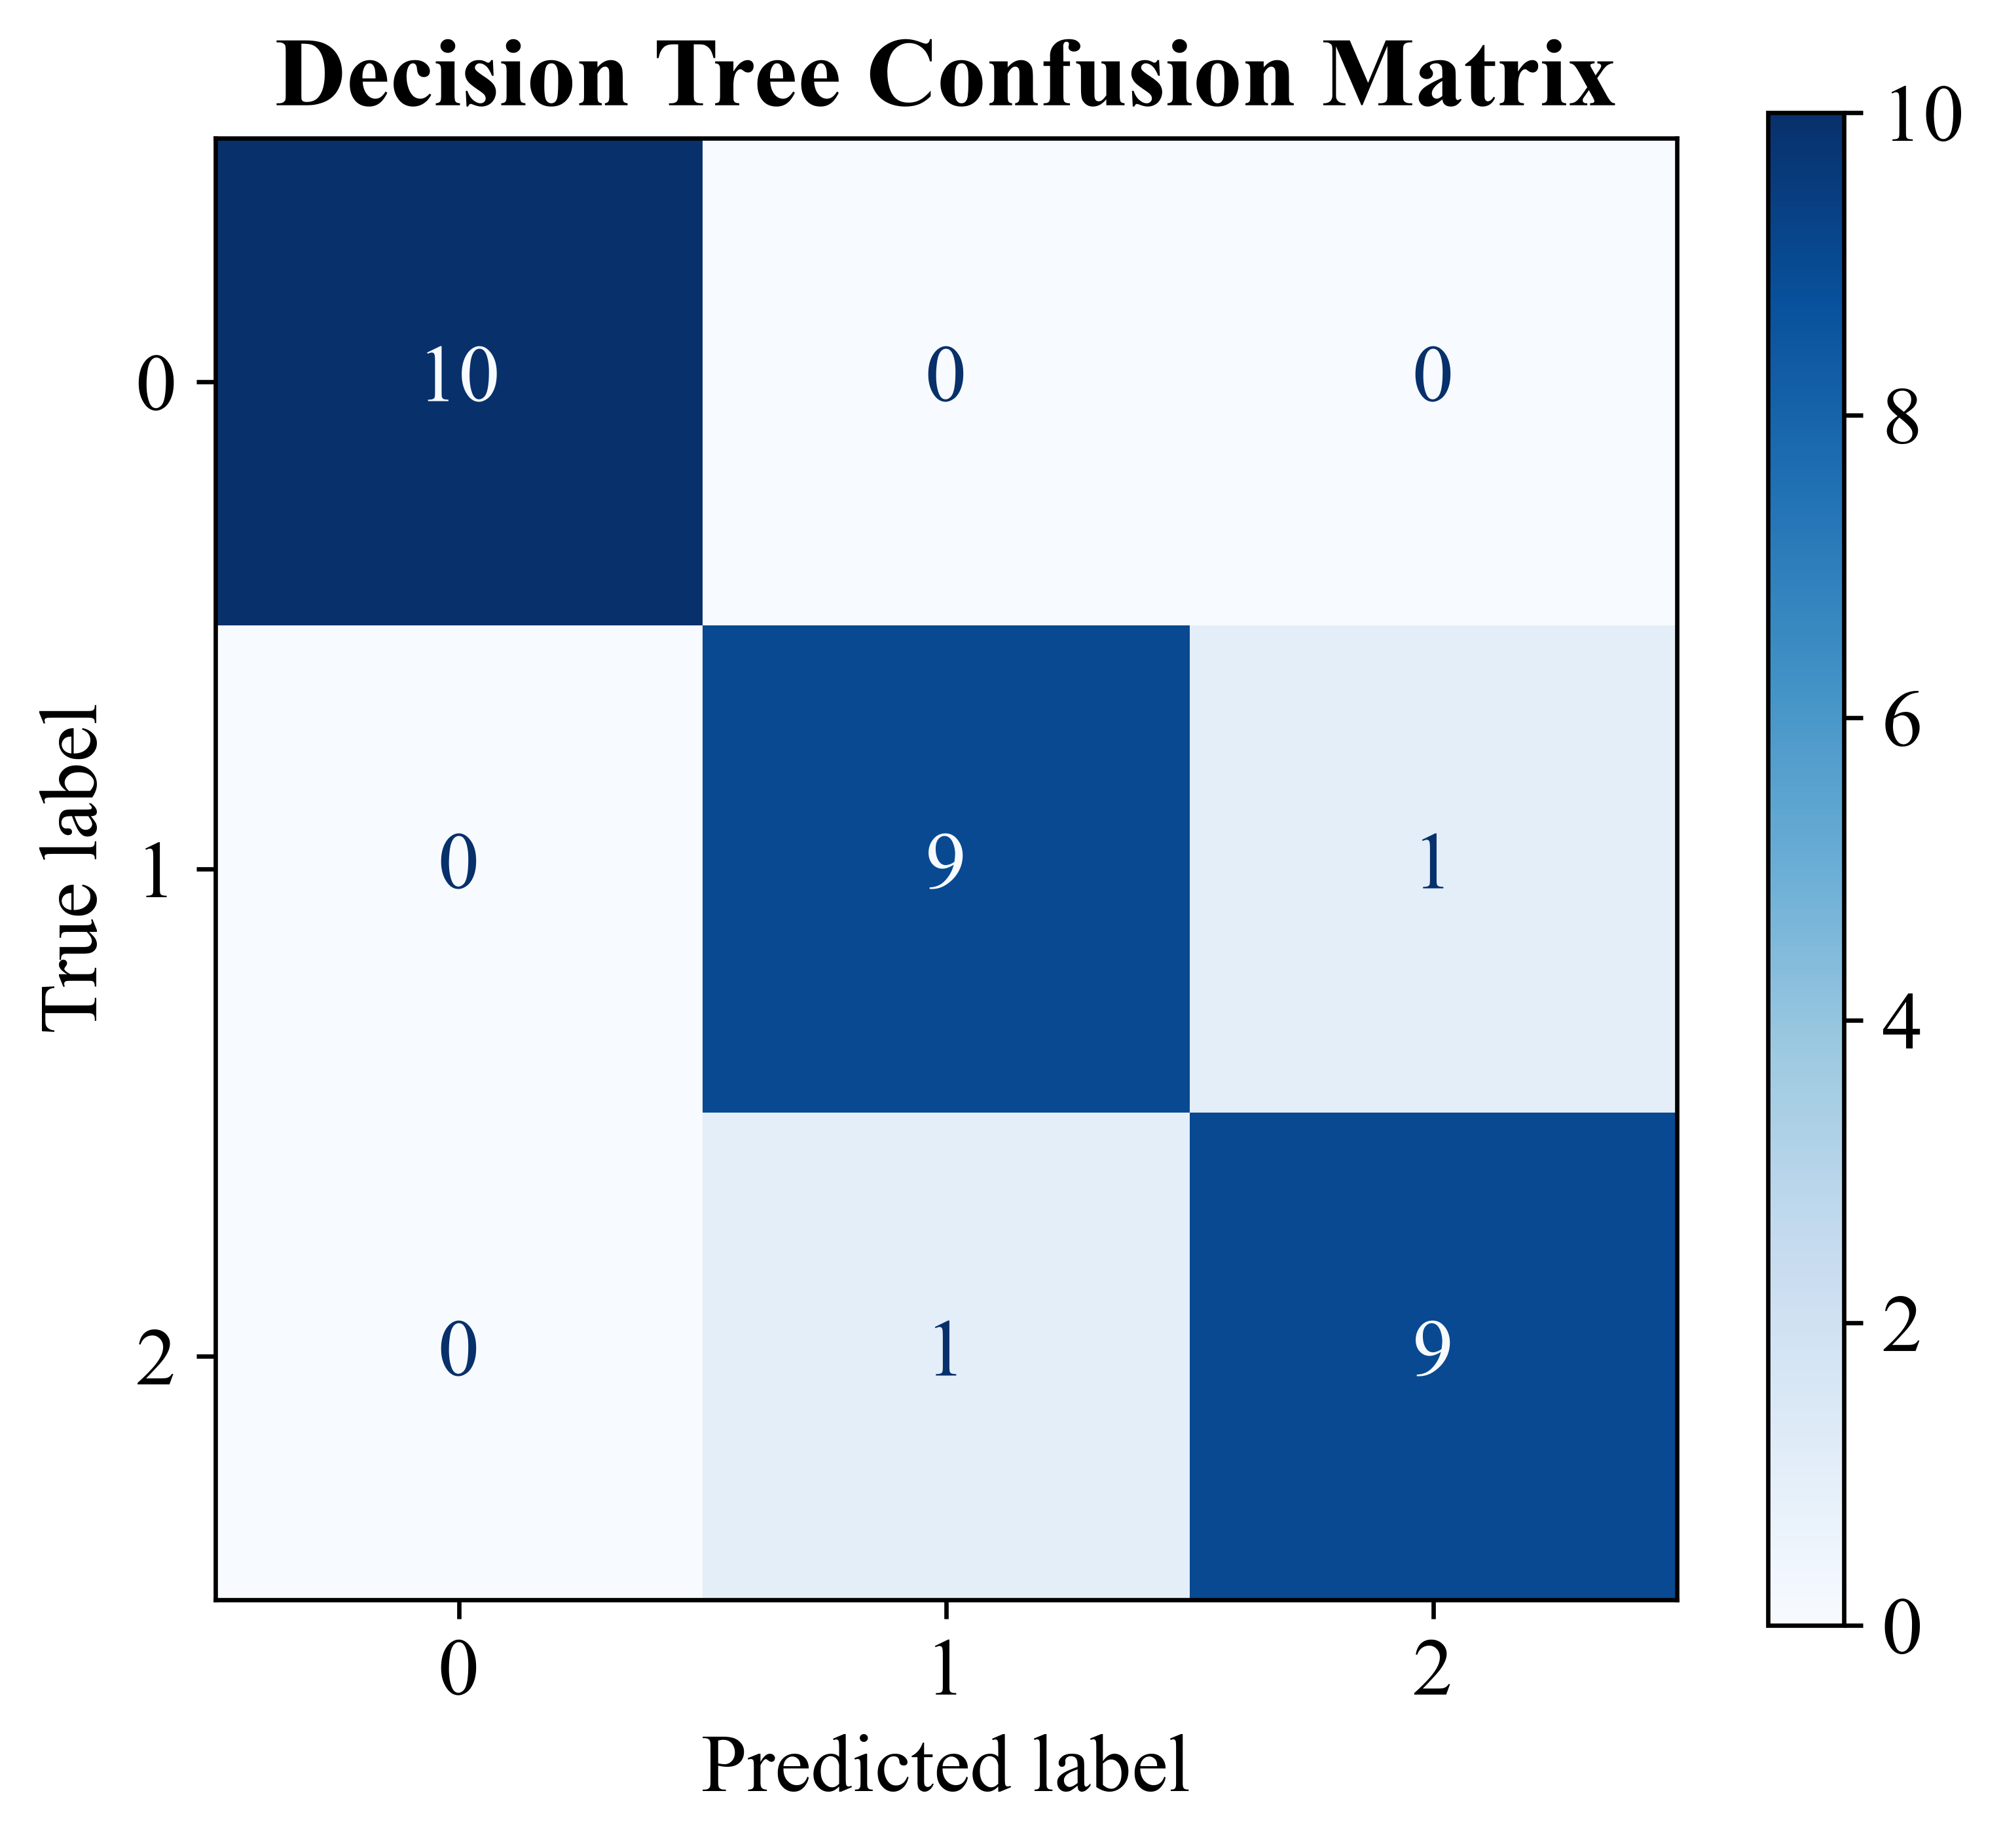
\includegraphics[width=0.55\linewidth]{decision_tree_confusion_matrix.png}
\caption{Confusion Matrix -- Decision Tree (Iris)}
\end{figure}

\textbf{Inference:} The single Decision Tree performs slightly worse than the ensemble methods (93.33\% accuracy), with confusion concentrated symmetrically between \textit{versicolor} and \textit{virginica} (one misclassification in each direction) -- the two species with known feature overlap in sepal measurements. This is the expected behavior of a single high-variance tree compared to an ensemble, which averages away exactly this kind of boundary-case instability.

\subsection*{K-Nearest Neighbors}

\begin{table}[H]
\centering
\begin{tabular}{lccc}
\toprule
Class & Precision & Recall & F1-Score \\
\midrule
0 (setosa) & 1.00 & 1.00 & 1.00 \\
1 (versicolor) & 0.83 & 1.00 & 0.91 \\
2 (virginica) & 1.00 & 0.80 & 0.89 \\
\bottomrule
\end{tabular}
\caption{KNN -- Classification Report (Iris)}
\end{table}

Confusion Matrix: $\begin{bmatrix} 10 & 0 & 0 \\ 0 & 10 & 0 \\ 0 & 2 & 8 \end{bmatrix}$

\begin{figure}[H]
\centering
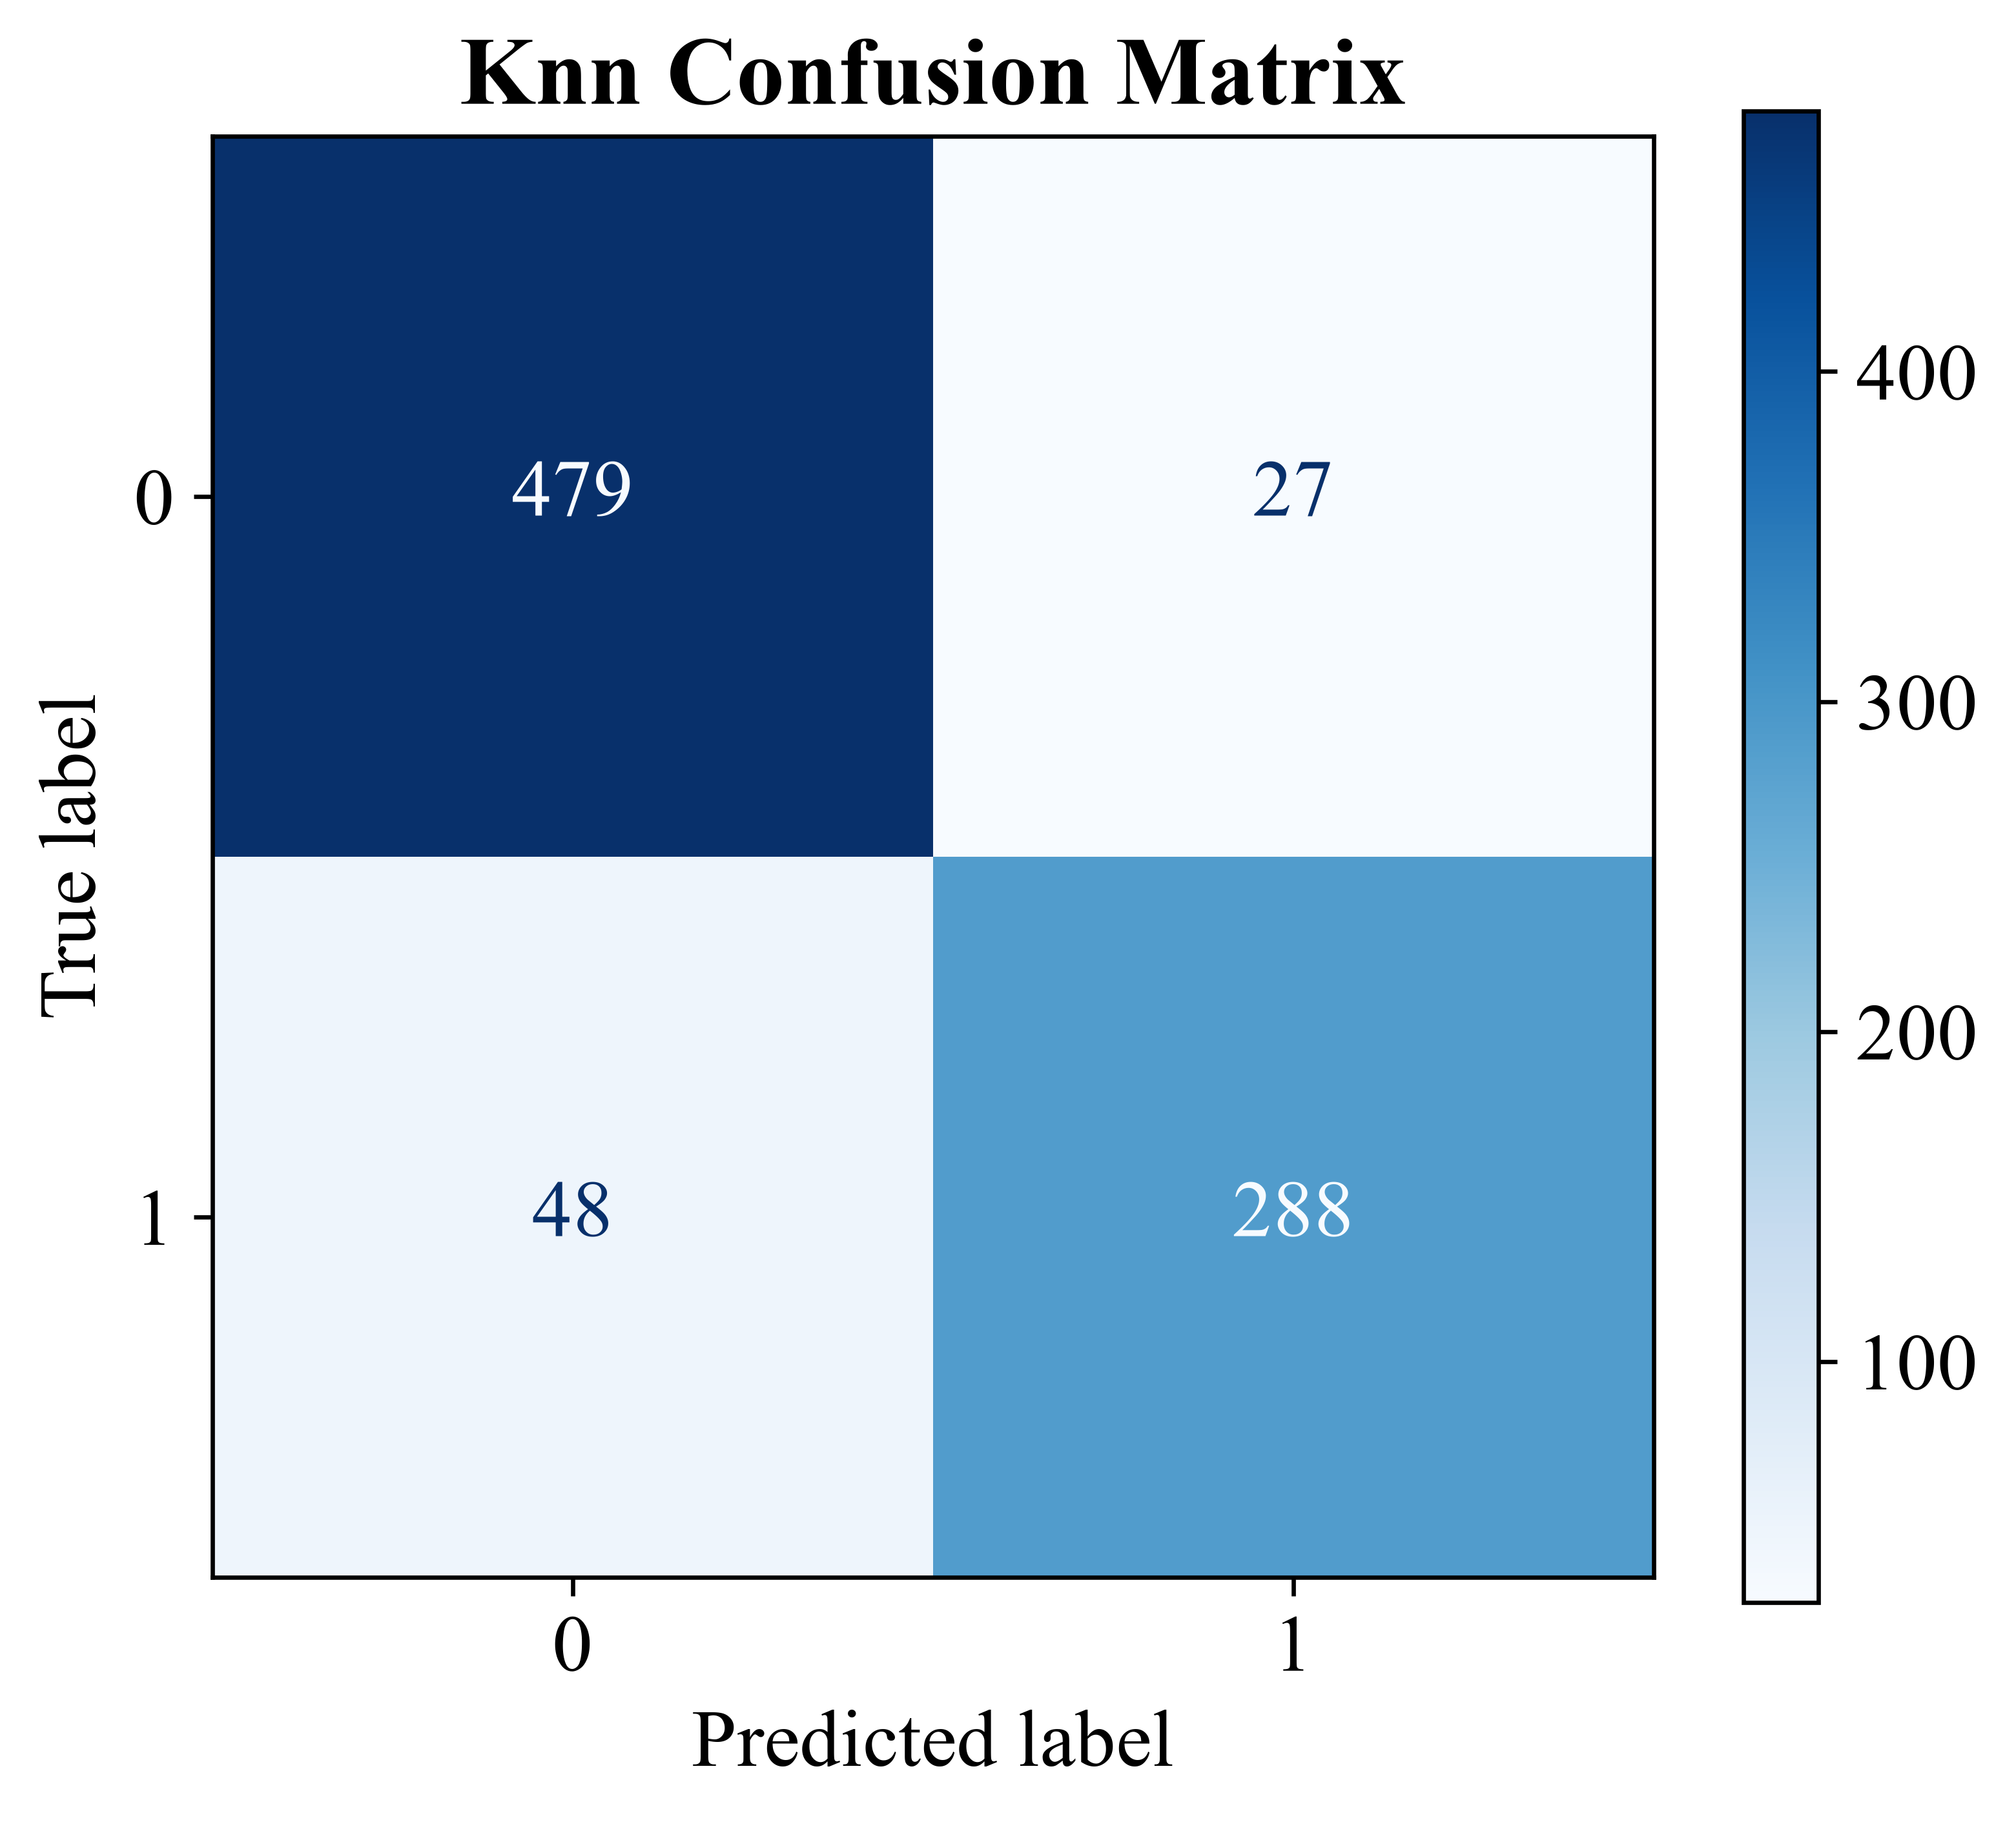
\includegraphics[width=0.55\linewidth]{knn_confusion_matrix.png}
\caption{Confusion Matrix -- KNN (Iris)}
\end{figure}

\textbf{Inference:} KNN achieves the highest ROC-AUC among all four models (0.9933) despite a slightly lower raw accuracy than Random Forest and SVM, indicating strong class-separation confidence in its distance-based decision function even where 2 \textit{virginica} samples are misclassified as \textit{versicolor}. This reflects that scaling the features prior to distance computation (per the preprocessing formula above) was effective in making Euclidean distance a meaningful similarity measure.

\subsection*{Support Vector Machine}

\begin{table}[H]
\centering
\begin{tabular}{lccc}
\toprule
Class & Precision & Recall & F1-Score \\
\midrule
0 (setosa) & 1.00 & 1.00 & 1.00 \\
1 (versicolor) & 1.00 & 0.90 & 0.95 \\
2 (virginica) & 0.91 & 1.00 & 0.95 \\
\bottomrule
\end{tabular}
\caption{SVM -- Classification Report (Iris)}
\end{table}

Confusion Matrix: $\begin{bmatrix} 10 & 0 & 0 \\ 0 & 9 & 1 \\ 0 & 0 & 10 \end{bmatrix}$

\begin{figure}[H]
\centering
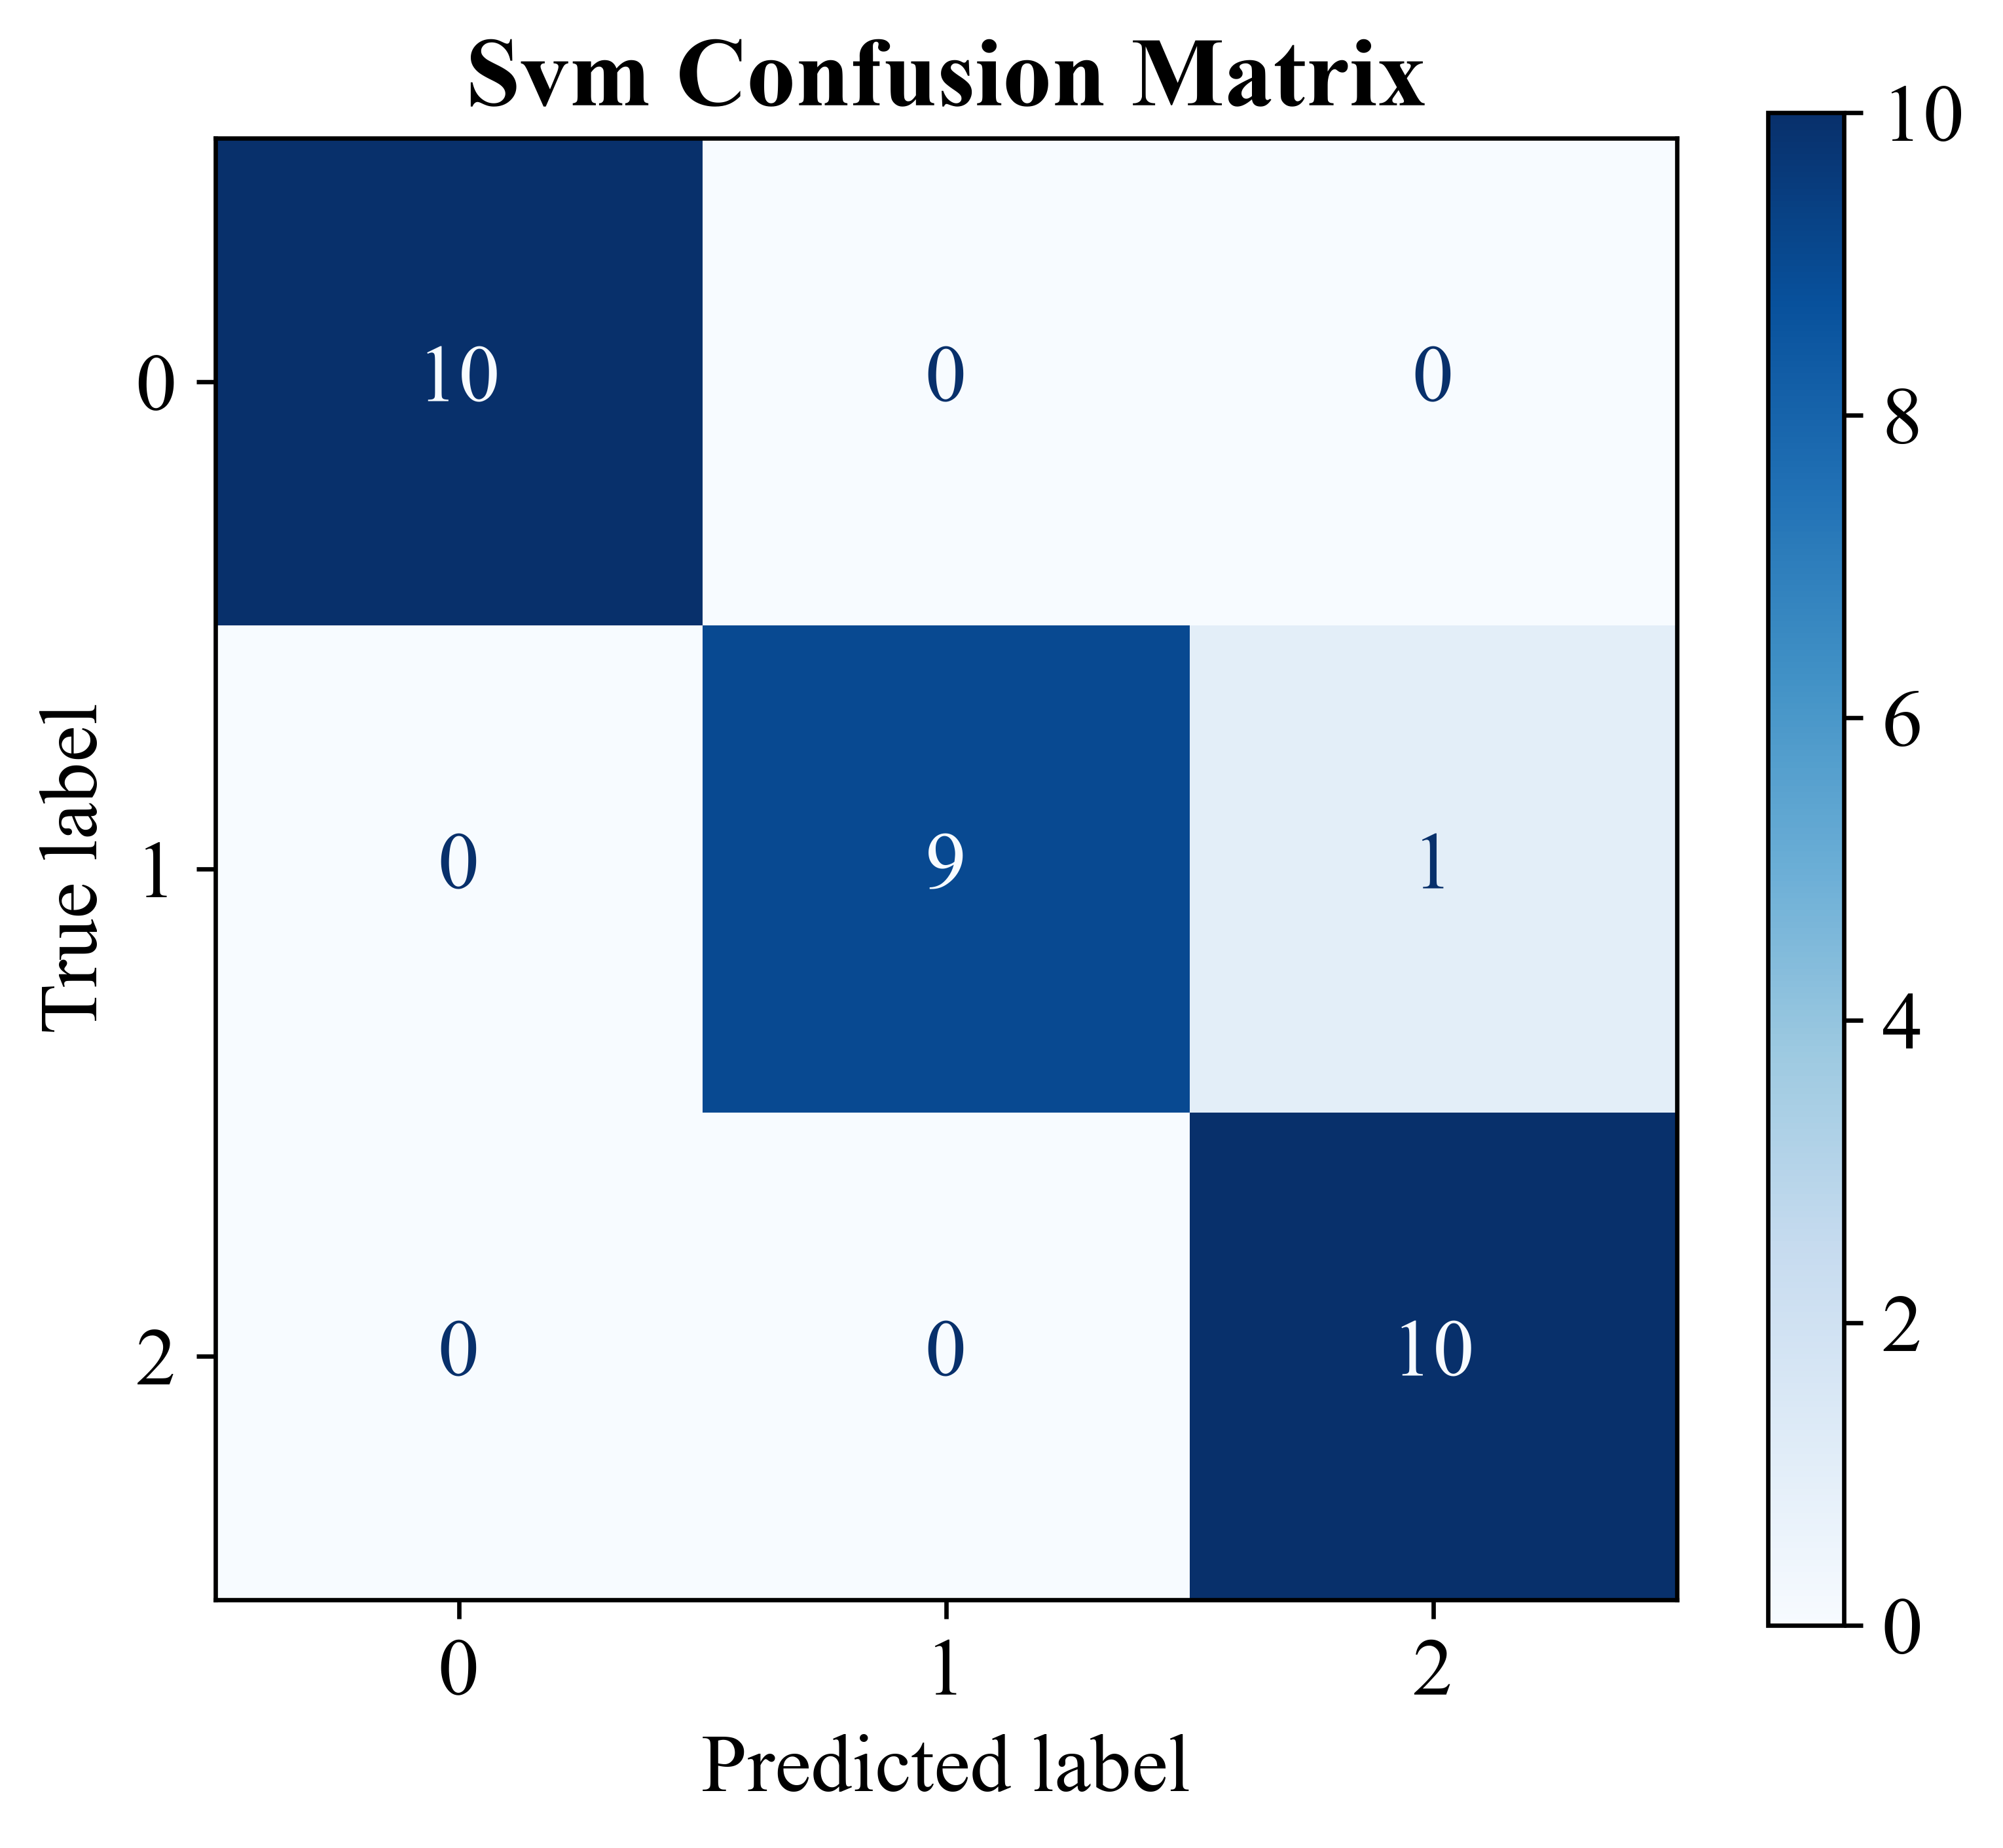
\includegraphics[width=0.55\linewidth]{svm_confusion_matrix.png}
\caption{Confusion Matrix -- SVM (Iris)}
\end{figure}

\textbf{Inference:} SVM matches Random Forest's accuracy (96.67\%) and achieves the highest ROC-AUC of all four models (0.9967), confirming that a margin-maximizing hyperplane (with kernel mapping where necessary) separates the three Iris species almost perfectly on this small, well-behaved, near-linearly-separable dataset.

\section{Results -- Diabetes Dataset}

The Diabetes dataset was evaluated using the \texttt{run\_pipeline()} function with a Random Forest classifier and ANOVA feature selection.

\begin{table}[H]
\centering
\begin{tabular}{lc}
\toprule
Metric & Value \\
\midrule
Accuracy & 0.7403 \\
Accuracy (\%) & 74.03\% \\
\bottomrule
\end{tabular}
\caption{Diabetes Dataset -- Random Forest Performance}
\end{table}

\begin{table}[H]
\centering
\begin{tabular}{lcccc}
\toprule
Class & Precision & Recall & F1-Score & Support \\
\midrule
0 (Non-Diabetic) & 0.82 & 0.77 & 0.79 & 99 \\
1 (Diabetic) & 0.62 & 0.69 & 0.66 & 55 \\
\midrule
Macro Avg & 0.72 & 0.73 & 0.72 & 154 \\
Weighted Avg & 0.75 & 0.74 & 0.74 & 154 \\
\bottomrule
\end{tabular}
\caption{Diabetes Dataset -- Classification Report}
\end{table}

Confusion Matrix: $\begin{bmatrix} 76 & 23 \\ 17 & 38 \end{bmatrix}$

Using the confusion matrix above with the positive class defined as Diabetic (1): $TP = 38$, $TN = 76$, $FP = 23$, $FN = 17$. Substituting into the formulas from Section 8:
\[
\text{Accuracy} = \frac{38+76}{38+76+23+17} = \frac{114}{154} = 0.7403
\]
\[
\text{Precision} = \frac{38}{38+23} = 0.6230, \qquad \text{Recall} = \frac{38}{38+17} = 0.6909
\]
\[
\text{F1-Score} = 2\cdot\frac{0.6230 \times 0.6909}{0.6230+0.6909} = 0.6552
\]
(these match, up to rounding, the class-1 row of the classification report above).

\textbf{Inference:} The Random Forest model achieves 74.03\% accuracy on the Diabetes test set, noticeably lower than the accuracy achieved on the Iris dataset. This is expected given the greater class imbalance (65\%/35\%) and inherent medical variability of the Diabetes dataset. The classification report and the worked calculation above show the model is more reliable at identifying non-diabetic patients (precision 0.82) than diabetic patients (precision 0.62), with 23 non-diabetic patients misclassified as diabetic and 17 diabetic patients missed (false negatives) -- a trade-off that would need to be tuned via class weighting or threshold adjustment in a real clinical screening application, where minimizing false negatives is typically prioritized.

\section{Discussion}

This experiment validated a single, reusable machine learning pipeline across two datasets with different sizes, feature counts, and class structures, while also grounding each modeling and evaluation step in its underlying mathematical formulation. On the well-separated, balanced, low-dimensional Iris dataset, all four classifiers achieved strong performance (93--97\% accuracy), with the margin-based SVM and ensemble-based Random Forest both reaching the highest accuracy (96.67\%) and ROC-AUC scores above 0.99. This is consistent with the EDA finding that Iris petal measurements provide near-linear separability between classes, which favors both the Gini-impurity-driven splits of tree ensembles and the maximum-margin hyperplane of SVM equally.

On the larger, moderately imbalanced Diabetes dataset, the same style of pipeline (Random Forest with ANOVA feature selection) achieved a considerably lower accuracy of 74.03\%, reflecting the genuinely higher difficulty and noisier feature-target relationships typical of real-world medical data compared to the classical, well-curated Iris benchmark. The worked precision/recall/F1 calculation confirms that accuracy alone masks a meaningful asymmetry: the model is a stronger predictor of the majority (non-diabetic) class than of the diabetic class, a pattern typical of moderately imbalanced binary classification problems and one that class-weighting or resampling could help address. The experiment confirms that library familiarity, a reusable pipeline design, and a clear grasp of the mathematics behind each algorithm and metric together are sufficient to obtain and correctly interpret reasonable baseline results across diverse classification problems.

\section{Conclusion}

This experiment successfully explored the core Python ML libraries -- NumPy, Pandas, SciPy, Scikit-learn, and Matplotlib -- through a unified, reusable machine learning workflow applied to both the Iris and Diabetes datasets, with each preprocessing step, algorithm, and evaluation metric grounded in its formal mathematical definition. On the Iris dataset, Random Forest and SVM jointly achieved the best test accuracy (96.67\%), with SVM achieving the highest ROC-AUC (0.9967). On the Diabetes dataset, a Random Forest model trained through the same style of pipeline achieved a test accuracy of 74.03\%, with a corresponding classification report and worked metric calculations highlighting the greater difficulty of the imbalanced, real-world medical prediction task. The experiment confirms the practicality of a single, well-modularized pipeline for rapid experimentation across datasets of different scale and difficulty, forming the foundation for the more advanced regression and classification experiments in this laboratory series.

\section{References}

\begin{enumerate}
\item C. M. Bishop, \textit{Pattern Recognition and Machine Learning}, Springer, 2006.
\item T. Hastie, R. Tibshirani, and J. Friedman, \textit{The Elements of Statistical Learning}, 2nd ed., Springer, 2009.
\item S. Raschka and V. Mirjalili, \textit{Python Machine Learning}, 3rd ed., Packt Publishing, 2019.
\item F. Pedregosa et al., ``Scikit-learn: Machine Learning in Python,'' \textit{Journal of Machine Learning Research}, vol. 12, pp. 2825--2830, 2011.
\item R. A. Fisher, ``The Use of Multiple Measurements in Taxonomic Problems,'' \textit{Annals of Eugenics}, vol. 7, no. 2, pp. 179--188, 1936.
\item J. W. Smith et al., ``Using the ADAP Learning Algorithm to Forecast the Onset of Diabetes Mellitus,'' \textit{Proceedings of the Symposium on Computer Applications in Medical Care}, 1988.
\item L. Breiman, ``Random Forests,'' \textit{Machine Learning}, vol. 45, no. 1, pp. 5--32, 2001.
\item Scikit-learn Documentation, \url{https://scikit-learn.org/}
\end{enumerate}

\section*{Appendix}

\subsection*{A.1 Implementation Details}

The experiment was implemented using Python with reusable modules for:
\begin{itemize}
\item Data loading and inspection (\texttt{data\_loader.py}, \texttt{utils.py})
\item EDA (\texttt{eda.py})
\item Preprocessing pipeline (\texttt{preprocessing.py})
\item Feature selection (\texttt{feature\_selection.py})
\item Classification model training (\texttt{classification.py})
\item Performance evaluation (\texttt{metrics.py})
\item End-to-end pipeline execution (\texttt{main.py})
\end{itemize}

\subsection*{A.2 Library Versions}

\begin{lstlisting}
NumPy:        1.26.4
Pandas:       2.2.2
SciPy:        1.13.1
Scikit-learn: 1.4.2
\end{lstlisting}

\subsection*{A.3 Environment Activation Command}

\begin{lstlisting}
source /opt/anaconda3/bin/activate anaconda-navigation
\end{lstlisting}

\end{document}